% !TeX spellcheck = en_GB
%%%%%%%%%%%%%%%%%%%%%%%%%%%%%%%%%%%%%%%%%
% Masters/Doctoral Thesis 
% LaTeX Template
% Version 2.5 (27/8/17)
%
% This template was downloaded from:
% http://www.LaTeXTemplates.com
%
% Version 2.x major modifications by:
% Vel (vel@latextemplates.com)
%
% This template is based on a template by:
% Steve Gunn (http://users.ecs.soton.ac.uk/srg/softwaretools/document/templates/)
% Sunil Patel (http://www.sunilpatel.co.uk/thesis-template/)
%
% Template license:
% CC BY-NC-SA 3.0 (http://creativecommons.org/licenses/by-nc-sa/3.0/)
%
%%%%%%%%%%%%%%%%%%%%%%%%%%%%%%%%%%%%%%%%%

%----------------------------------------------------------------------------------------
%   PACKAGES AND OTHER DOCUMENT CONFIGURATIONS
%----------------------------------------------------------------------------------------

\documentclass[
12pt, % The default document font size, options: 10pt, 11pt, 12pt
oneside, % Two side (alternating margins) for binding by default, uncomment to switch to one side
english, % ngerman for German
onehalfspacing, % Single line spacing, alternatives: onehalfspacing or doublespacing
%draft, % Uncomment to enable draft mode (no pictures, no links, overfull hboxes indicated)
nolistspacing, % If the document is onehalfspacing or doublespacing, uncomment this to set spacing in lists to single
%liststotoc, % Uncomment to add the list of figures/tables/etc to the table of contents
%toctotoc, % Uncomment to add the main table of contents to the table of contents
%parskip, % Uncomment to add space between paragraphs
%nohyperref, % Uncomment to not load the hyperref package
%headsepline, % Uncomment to get a line under the header
chapterinoneline, % Uncomment to place the chapter title next to the number on one line
%consistentlayout, % Uncomment to change the layout of the declaration, abstract and acknowledgements pages to match the default layout
]{MastersDoctoralThesis} % The class file specifying the document structure

\usepackage[utf8]{inputenc} % Required for inputting international characters
\usepackage[T1]{fontenc} % Output font encoding for international characters
\usepackage{changepage}
\usepackage{textcomp}
\usepackage[a-1b]{pdfx}
\usepackage{mathpazo} % Use the Palatino font by default

\usepackage[backend=bibtex,style=ieee ]{biblatex} % Use the bibtex backend with the authoryear citation style (which resembles APA)

\addbibresource{references.bib} % The filename of the bibliography

\usepackage[autostyle=true]{csquotes} % Required to generate language-dependent quotes in the bibliography
\usepackage[outdir=./]{epstopdf}
\usepackage{graphicx}
\usepackage{amsmath}
\usepackage{amsfonts}
\usepackage{todonotes}
\usepackage{subfig}
\usepackage{minted}
\usemintedstyle{pastie}
\usepackage{enumitem}
\usepackage{svg}
\usepackage{blkarray}
\usepackage{booktabs} 
\usepackage{colortbl} 
\usepackage{xcolor} 
\usepackage{xfrac}
\usepackage{siunitx}
\usepackage{caption}

\usepackage{subfig}


\captionsetup[figure]{width=.85\textwidth}
\captionsetup[subfigure]{margin=0pt}
\setminted{
    linenos=true,
    autogobble,
}
\newenvironment{longlisting}{\captionsetup{type=listing}}{}
\setcounter{MaxMatrixCols}{20}
\setcounter{tocdepth}{2}
\reversemarginpar
\graphicspath{ {Figures/} }
\graphicspath{ {../matlab/} }
%----------------------------------------------------------------------------------------
%   MARGIN SETTINGS
%------------------------------------------------
% ----------------------------------------

\geometry{
    paper=a4paper, % Change to letterpaper for US letter
    inner=4.5cm, % Inner margin
    outer=2cm, % Outer margin
    bindingoffset=.5cm, % Binding offset
    top=2.5cm, % Top margin
    bottom=3cm, % Bottom margin
    %showframe, % Uncomment to show how the type block is set on the page
}

%----------------------------------------------------------------------------------------
%   THESIS INFORMATION
%----------------------------------------------------------------------------------------

\thesistitle{Fuzzy logic and unmanned surface vehicles} % Your thesis title, this is used in the title and abstract, print it elsewhere with \ttitle
\thesissubtitle{Implementing collision avoidance in Python}

\supervisor{Prof. Johan \textsc{Lilius} \\ Adj. Prof. Marina \textsc{Waldén} } % Your supervisor's name, this is used in the title page, print it elsewhere with \supname
\examiner{} % Your examiner's name, this is not currently used anywhere in the template, print it elsewhere with \examname
\degree{Master of Science (Technology)} % Your degree name, this is used in the title page and abstract, print it elsewhere with \degreename
\author{Emil \textsc{Aura}} % Your name, this is used in the title page and abstract, print it elsewhere with \authorname
\addresses{} % Your address, this is not currently used anywhere in the template, print it elsewhere with \addressname

\subject{Biological Sciences} % Your subject area, this is not currently used anywhere in the template, print it elsewhere with \subjectname
\keywords{COLREGS, Unmanned Surface Vessels, Fuzzy Logic} % Keywords for your thesis, this is not currently used anywhere in the template, print it elsewhere with \keywordnames
\university{\href{http://www.abo.no}{Åbo Akademi University}} % Your university's name and URL, this is used in the title page and abstract, print it elsewhere with \univname
\department{\href{https://research.it.abo.fi/}{Department of Information Technologies}} % Your department's name and URL, this is used in the title page and abstract, print it elsewhere with \deptname
\group{\href{https://uit.no/utdanning/program?p_document_id=275406}{University of Tromsø School of Aviation}} % Your research group's name and URL, this is used in the title page, print it elsewhere with \groupname
\faculty{\href{http://www.abo.fi/fakultet/en/fnt}{Faculty of Science and Engineering}} % Your faculty's name and URL, this is used in the title page and abstract, print it elsewhere with \facname

\AtBeginDocument{
\hypersetup{pdftitle=\ttitle - \tsubtitle} % Set the PDF's title to your title
\hypersetup{pdfauthor=\authorname} % Set the PDF's author to your name
\hypersetup{pdfkeywords=\keywordnames} % Set the PDF's keywords to your keywords
}

\hypersetup{pdfencoding=unicode}

\begin{document}


\frontmatter % Use roman page numbering style (i, ii, iii, iv...) for the pre-content pages

\pagestyle{plain} % Default to the plain heading style until the thesis style is called for the body content

%----------------------------------------------------------------------------------------
%   TITLE PAGE
%----------------------------------------------------------------------------------------
\newgeometry{ inner=2cm, % Inner margin
    outer=2cm, % Outer margin
    top=2cm, % Top margin
    bottom=2cm, % Bottom margin} 
}
\begin{titlepage}
    \thispagestyle{author}
    % \begin{adjustwidth}{-2.0cm}{-2.0cm}
    
\includegraphics[width=40mm]{Figures/Logo_eng_pos.pdf}
    %   \end{adjustwidth} 
    % thesis title centered and in big bold fonts
    \begin{center}
        \LARGE\textbf{\ttitle} \\
        \textit{\tsubtitle}
        \par

        % thesis author name and matriculation number below in normal text
        {\large

            \vspace{5mm}
            \begin{tabular}[t]{c}
                \authorname
                %\thesisauthormatrnr         
            \end{tabular}}
        \par

    \end{center}
    \vfill
    \begin{bottompar}

        %\begin{adjustwidth}{-2.0cm}{-2.0cm}
        \begin{flushright}
            \ifdefined\swedishthesis
                Bachelor's thesis  \\
                %Handledare: \thesissupervisor \\
                %\ifdefined\examinerspecified
                %�vervakare: \thesisexaminer
                %\fi
            \else
                Master's thesis (30 ECTS)  \\
                Supervisors: \supname \\
            \fi
            \deptname \\
            \facname \\
            \univname \\
            \today\\% Date
            \vspace{5 mm}
            {\fontsize{8pt}{1em}\selectfont Åbo Akademi University, Tuomiokirkontori 3 , FI-20500 TURKU  ~/ +358 2 215 31 / information@abo.fi  / \href{http://abo.fi}{abo.fi}
                % 
\includegraphics[width=15mm]{Figures/Logo_eng_pos.pdf}
            }
        \end{flushright}
        % \end{adjustwidth} 
    \end{bottompar}

\end{titlepage}
\restoregeometry


%----------------------------------------------------------------------------------------
%   DECLARATION PAGE
%----------------------------------------------------------------------------------------

%\begin{declaration}
% \addchaptertocentry{\authorshipname} % Add the declaration to the table of contents
% \noindent I, \authorname, declare that this thesis titled, \enquote{\ttitle} and the work presented in it are my own. I confirm that:

% \begin{itemize} 
% \item This work was done wholly or mainly while in candidature for a research degree at this University.
% \item Where any part of this thesis has previously been submitted for a degree or any other qualification at this University or any other institution, this has been clearly stated.
% \item Where I have consulted the published work of others, this is always clearly attributed.
% \item Where I have quoted from the work of others, the source is always given. With the exception of such quotations, this thesis is entirely my own work.
% \item I have acknowledged all main sources of help.
% \item Where the thesis is based on work done by myself jointly with others, I have made clear exactly what was done by others and what I have contributed myself.\\
% \end{itemize}

% \noindent Signed:\\
% \rule[0.5em]{25em}{0.5pt} % This prints a line for the signature

% \noindent Date:\\
% \rule[0.5em]{25em}{0.5pt} % This prints a line to write the date
%\end{declaration}

\cleardoublepage

%----------------------------------------------------------------------------------------
%   QUOTATION PAGE
%----------------------------------------------------------------------------------------

%\vspace*{0.2\textheight}

%\noindent\enquote{\itshape Thanks to my solid academic training, today I can write hundreds of words on virtually any topic without possessing a shred of information, which is how I got a good job in journalism.}\bigbreak

%\hfill Dave Barry

%----------------------------------------------------------------------------------------
%   ABSTRACT PAGE
%----------------------------------------------------------------------------------------

\begin{abstract}
    \addchaptertocentry{\abstractname} % Add the abstract to the table of contents
    Autonomous vessels could potentially  lower the costs of maritime shipping, by reducing the operating costs and increasing the safety.
    However, one of the greater challenges in the pursuit of completely autonomous and unmanned vessels lies in  the development of algorithms capable of making decisions as safe and efficient as human operators.
    The purpose of this thesis is to evaluate the use of fuzzy logic in a COLREGS compliant collision avoidance algorithm, for unmanned surface vessels. A python implementation utilizing a fuzzy logic inference system is developed and tested in simultations of maritime scenarios involving multiple vessels.

    Results show the algorithm capable of avoiding collisions, although further work is needed to make the algorithm truly COLREGS compliant and the decisions more holistic.
    \\\\
    \textit{Keywords:} \textit{\keywordnames}
\end{abstract}

%----------------------------------------------------------------------------------------
%   ACKNOWLEDGEMENTS
%----------------------------------------------------------------------------------------

\begin{acknowledgements}


    \addchaptertocentry{\acknowledgementname} % Add the acknowledgements to the table of contents
    I would like to thank my advisor Professor Johan Lilius for giving me the opportunity to write this thesis and for helping me to steer back to course when my thesis was drifting on the oceans of academia. I'd also like to thank Adjunct Professor Marina Waldén for all the feedback during the writing process. Thanks also go to Annamari Soini for starting the process by putting me in contact with the right people.

    \vspace{2cm}

    \noindent Emil Aura\\
    Turku, \today

\end{acknowledgements}
%----------------------------------------------------------------------------------------
%   LIST OF CONTENTS/FIGURES/TABLES PAGES
%----------------------------------------------------------------------------------------

\tableofcontents % Prints the main table of contents
\setcounter{tocdepth}{1}
\listoffigures % Prints the list of figures

\listoftables % Prints the list of tables


%----------------------------------------------------------------------------------------
%   ABBREVIATIONS
%----------------------------------------------------------------------------------------

\begin{abbreviations}{l p{10cm}} % Include a list of abbreviations (a table of two columns)
    \textbf{COLREGs}  & Convention on the International Regulations for Preventing Collisions at Sea, 1972\\
    \textbf{FMF} & \textbf{F}uzzy \textbf{M}embership \textbf{F}unction\\
    \textbf{OPRA} & \textbf{O}riented \textbf{P}oint \textbf{R}easoning \textbf{A}lgebra\\
    \textbf{SA} & \textbf{S}ituational \textbf{A}wareness\\
    \textbf{FIS} & \textbf{F}uzzy \textbf{I}nference \textbf{S}ystem\\

\end{abbreviations}

%----------------------------------------------------------------------------------------
%   PHYSICAL CONSTANTS/OTHER DEFINITIONS
%----------------------------------------------------------------------------------------

% \begin{constants}{lr@{${}={}$}l} % The list of physical constants is a three column table

% % The \SI{}{} command is provided by the siunitx package, see its documentation for instructions on how to use it

% Speed of Light & $c_{0}$ & \SI{2.99792458e8}{\meter\per\second} (exact)\\
% %Constant Name & $Symbol$ & $Constant Value$ with units\\

% \end{constants}

%----------------------------------------------------------------------------------------
%   SYMBOLS
%----------------------------------------------------------------------------------------

% \begin{symbols}{lll} % Include a list of Symbols (a three column table)

% $a$ & distance & \si{\meter} \\
% $P$ & power & \si{\watt} (\si{\joule\per\second}) \\
% %Symbol & Name & Unit \\

% \addlinespace % Gap to separate the Roman symbols from the Greek

% $\omega$ & angular frequency & \si{\radian} \\

% \end{symbols}

%----------------------------------------------------------------------------------------
%   DEDICATION
%----------------------------------------------------------------------------------------

% \dedicatory{For/Dedicated to/To my\ldots} 

%----------------------------------------------------------------------------------------
%   THESIS CONTENT - CHAPTERS
%----------------------------------------------------------------------------------------

\mainmatter % Begin numeric (1,2,3...) page numbering

\pagestyle{thesisSimple} % Return the page headers back to the "thesis" style

% Include the chapters of the thesis as separate files from the Chapters folder
% Uncomment the lines as you write the chapters

%!TEX root = ../main.tex
% !TeX spellcheck = en_GB 

% Chapter 1

\chapter{Introduction} % Main chapter title

\label{Introduction} % For referencing the chapter elsewhere, use \ref{Chapter1} 

%----------------------------------------------------------------------------------------

% Define some commands to keep the formatting separated from the content 
\newcommand{\keyword}[1]{\textbf{#1}}
\newcommand{\tabhead}[1]{\textbf{#1}}
\newcommand{\code}[1]{\texttt{#1}}
\newcommand{\file}[1]{\texttt{\bfseries#1}}
\newcommand{\option}[1]{\texttt{\itshape#1}}

%----------------------------------------------------------------------------------------

Maritime shipping can be considered one of the pillars of the modern economy. In fact the \textcite{percent_trade} state that 90\% of the worlds total trade is handled by maritime shipping. This sums up to roughly 1 600 000 seafarers serving on international trading merchant ships worldwide. However, the recent rapid development of sensor technology and artificial intelligence could potentially reduce the operational costs of such vessels, by facilitating the developments of  Unmanned surface vehicles (USVs). The number of persons needed to operate vessels could thereby be reduced significantly. Furthermore, a majority of the accidents reported between 2011 and 2016 can be linked to human erroneous actions \cite{marine_casualities_incidents_2017}. USVs could, thus potentially decrease both the operational costs and the number of accidents.

It is therefore of utmost interest to overcome the challenges connected to the development of USVs. One of these challenges  is the development of algorithms to handle collision avoidance between vessels in agreement with the rules of navigation. Various approaches have already been tried. This thesis will further examine the use of  fuzzy logic in a collision avoidance algorithm for USVs.
\section{Purpose}
The basis for this research lies in the work done by \textcite{perera2012intelligent}. However, this thesis tries to further test previous findings by recreating the previous implementation in python instead of MatLab and testing the algorithm in more challenging simulation scenarios than before.

\section{Disposition}
This first chapter  provides  general information about the thesis along with background information on the topic. Furthermore, it presents the purpose of the thesis. Additional background information on USVs, as well as their advantages and challenges, are presented in chapter \ref{Unmanned_Surface_Vehicles}. Chapter \ref{sec_colreg} explains the International Regulations for Preventing Collisions
at Sea (COLREGs) and describes a few collision avoidance situations.  Previous approaches to automation of COLREGs rules are presented in chapter \ref{chap:aut_colregs} after which the theory for the fuzzy logic approach used in this thesis is thoroughly explained in chapter \ref{chap:fuzzy}. The implementation of the fuzzy logic based Autonomous Navigation System and the simulation framework is described in chapter \ref{chap_impl}. Chapter \ref{sec:evaluation} presents the simulation scenarios as well as results and evaluations of the simulations. The results from chapter \ref{sec:evaluation} are discussed in chapter \ref{chap:disc}. Finally, conclusions are provided in chapter \ref{chap:conc}.
%!TEX root = ../main.tex
% !TeX spellcheck = en_GB 
% Chapter 2
%------------------------------------------------------------------------------------
\chapter{Unmanned Surface Vehicles} % Main chapter title

\label{Unmanned_Surface_Vehicles} % For referencing the chapter elsewhere, use \ref{Chapter1}
%------------------------------------------------------------------------------------


Unmanned Surface Vehicles (USV) or Autonomous Surface Crafts (ASC) are vehicles operating the seas without a crew on-board.
USVs encompass both fully autonomous vehicles, from now on referred to as ASCs, and semi-autonomous vehicles.
Development of USVs has been ongoing for the last two decades \cite{manley2008unmanned}.
However, the majority of the USVs developed are of the semi-autonomous type \cite{liu2016unmanned,park2017development}, meaning that they depend on human intervention to some extent usually by a supervisor located on shore.
Although semi-autonomous USVs greatly increase the safety of the operating personnel \cite{liu2016unmanned}, they do not completely remove the need for human interaction.
Supervision of several semi-autonomous vehicles can be admittedly be handled by a single person, which significantly decreases the number of person-hours needed to accomplish a specific mission \cite{manley2008unmanned}.
The person-hours needed for surveillance could, however, be removed completely by a ASC.
It is, therefore, of great interest to overcome the challenges associated with ASCs.


%------------------------------------------------------------------------------------
\section{Usage}
\textcite{Yuh2011} mention that roughly two-thirds of the earth's surface is covered by water, with an average depth of the oceans being 3688 m \cite{depth_ocean}.
Thereby, adding up to a vast amount of explorable areas of which 95 \% is yet to be seen by human eyes \cite{explored_percentage}. Utilization of autonomous vehicles could notably facilitate the  exploration of these, yet unknown, areas.
Although ASCs are situated on the surface of the ocean they can greatly increase the efficiency of Unmanned Underwater Vehicles (UUV) by acting as a gateway between UUVs and services, such as GPS, not easily available in underwater environments \cite{liu2016unmanned}.

\textcite{liu2016unmanned} have, furthermore, compiled a list of potential applications of USVs, along with previous research on the topics.
The list is divided into five major categories: scientific research, environmental missions, ocean resource exploration, military use, and other applications.

\section{Advantages}
\todo{More advantages}
USVs have, apart from the obvious decrease in man hours, a few advantages over traditional manned vessels. The absence of humans on board means that facilities and resources such as canteens,  manned bridges, showers etc. are no longer needed. The weight saved increases the manoeuvrability and deployability and can also be used to increase the payload the vessel is able to carry. USVs can, furthermore, conduct longer and more hazardous voyages than manned vessels since the personnel is located safely on land. This has the additional benefit of decreasing the operational costs \cite{liu2016unmanned}.

%\subsection{Current state}
%------------------------------------------------------------------------------------
\section{Challenges}
Even though USVs bring many advantages to the maritime industry, there are still quite a few challenges that need to be solved. The following section presents some of these challenges and their relation to the scope of this thesis.


USVs should be able to operate in a highly variable environment, all over the world, in terms of climate, traffic density and communication channels available.  Algorithms and systems developed should, therefore, ideally be usable in all situations that might arise in this environment. This introduces challenges both hardware and software wise \cite{liu2016unmanned}. The limited scope of this thesis narrows the research to only the software related challenges with a focus on path planning, especially collision avoidance.

All vessels operating on water are bound to follow the international maritime "Rules of the Road" called the Convention on the International Regulations for Preventing Collisions at Sea, 1972 (COLREGs) explained in section \ref{sec_colreg}. This is also true for USVs, since they should be able to operate in situations that comprise both other USVs and manned vessels that follow the COLREGs rules. Furthermore, they should be able to  act in a safe manner in situations where other vessels, for some reason, are not complying with the COLREGs rules. Hence, it is crucial for the USVs to follow COLREGs to ensure safe operations.

COLREGs were originally introduced in 1972, to reduce the amount of collisions at sea. They are written to be interpreted by humans. Situations where multiple rules apply and contradict each other might therefore arise. These situations are usually solved with the use of good seamanship and human deduction. These aspects pose challenges when translating the COLREGs rules into computer understandable code \cite{benjamin2006method}.


%------------------------------------------------------------------------------------
\chapter{COLREG}
\label{sec_colreg}
The Convention on the International Regulations for Preventing Collisions at Sea, 1972 (COLREGs) were adopted 1972 and entered into force 1977 in it's original form. COLREGs consist of 38 rules, grouped into five different sections as is designed by the International Maritime Organization (IMO).
The original objective of COLREGs was to ensure traffic separation between maritime vessels in an increasingly populated environment back in 1972 and it is, therefore, sometimes referred to as the Rules of the Road for maritime vessels. COLREGs have since then been in use and is still mandatory to adhere to on international waters. However, a great deal has changed since the COLREGs initially entered into force and COLREGs has, therefore,
received amendments several times \cite{colreg_about_imo}.

National regulations might differ from the COLREGs to some extent. However, COLREGs mention that ‘Nothing in these Rules shall interfere with the operation of special rules made by an appropriate authority for roadsteads, harbours, rivers, lakes or inland waterways connected with the high seas and navigable by seagoing vessels.
Such special rules shall conform as closely as possible to these Rules.’ \cite{colreg}

%------------------------------------------------------------------------------------
The following sections will present the different parts of the COLREGs regulations, with emphasis on the parts related to manoeuvring a USV in international waters. Information in this subsection is taken from the official COLREGs regulations  \cite{colreg} if not otherwise specified. Part D and E will not be discussed further, since they are not of interest for the scope of this thesis. Moreover, rules that are not of interest for the scope of this thesis will not be mentioned.
%------------------------------------------------------------------------------------
\section{Part A General}

Part A consist of three rules and address general conditions when and to which vessels COLREGs apply. This includes all vessels navigating on high seas and all waters connected therewith. Additionally, it specifies that special rules regarding roadsteads, harbours, rivers, lakes or inland waterways connected with the high seas and navigable by seagoing vessels shall conform as closely as possible to these Rules (\textit{Rule1}). Furthermore words, such as vessel, power-driven vessel, sailing vessel, length, breadth, and other words used in the regulations are defined (\textit{Rule3}). Finally, it is stated that the COLREGs rules do not in any way free the vessel, owner, master or crew from responsibility to follow the rules and act according to the ordinary practice of seamen (\textit{Rule2}).

%------------------------------------------------------------------------------------
\section{Part B Steering and Sailing}
Part B is split up into three different sections. The first section consists of rules \todo{words or numerals} 4-10 and apply in any condition of visibility. Section II (rules 11-18) apply to vessels in sight of each other, while the last section consist of just one rule that specifies reduced visibility operations. It states that vessels should proceed at speeds appropriate to the circumstances and use radar to determine collision risks. Speed should be reduced to a minimum if a vessel can hear another vessels fog horn apparently forward of her beam (\textit{Rule19}).

Section I addresses how vessels shall operate in order to ensure proper situational awareness with emphasis on collision risk detection.  It is mandatory for  all vessels to at all times maintain proper look-out by sight and hearing and all other available means to ensure the best possible situational awareness (\textit{Rule5}) and use all means possible to determine if a risk of collision exists. This includes the use of radar equipment although caution should be exercised not to trust insufficient data. A collision is considered to be imminent when two vessel maintain constant compass bearings to each other over a prolonged time.
However, a constant bearing is only a sufficient condition for a collision risk, not a necessary one. Close range, large vessels or a tow might pose a collision risk without a constant bearing. Moreover, it is stated that any doubt whether a risk of collision exists shall be treated as if a risk exists (\textit{Rule7}).
Vessels shall, furthermore, maintain a speed so that they can take proper and effective action to avoid a collision and stop within a distance appropriate to the prevailing circumstances and conditions (\textit{Rule 6}). Any actions made in order to to avoid collisions shall, additionally, be taken according to the rules and as far as possible be conducted in ample time and large enough so that they are easily observable by other vessels. Small alterations should, in other words, be avoided. Course alterations might also be accompanied by a lowering of speed, if considered necessary to ensure that the vessels pass each other at safe distance (\textit{Rule 8}).

Section II defines three different scenarios, involving two vessels, and specifies the action to take for both vessel. The scenarios are a head-on, a crossing and an overtake situation. A vessel overtaking another vessel shall keep out of the way of the stand on vessel. A vessel is considered to overtake another vessel when approaching it from a direction more than 22.5 \textdegree abaft the stand on vessels beam, i.e with a relative bearing between 112,5 \textdegree and 247,5 \textdegree from the stand on vessel (\textit{Rule 13}). A head-on situation, on the other hand, is when a vessel sees another vessel ahead or nearly ahead, i.e. it can see the masthead light in line or both sidelights. The give way vessel shall, in this case, alter its course to starboard (\textit{Rule 14}). Finally it is stated that vessel coming from starboard, i.e right, has the right of way in a crossing situation. The give way vessel shall if possible avoid crossing ahead of the other vessel and, therefore, alter its course to starboard  (\textit{Rule 15}). All actions by the give away vessels shall be taken as early as possible  (\textit{Rule 16}), while the stand on vessels shall keep its course and speed, provided that the give way vessel acts according to the regulations. However, the stand on vessel might take action to best avoid a collision if it finds that the actions by the give way vessels are insufficient to prevent a collision  (\textit{Rule 17}). Responsibilities between vessels of different types are also addressed. For instance, a power-driven vessel shall give way for vessels engaged in fishing,  vessels not under command,  vessels restricted in her ability to move, and finally fishing vessels   (\textit{Rule 18}).

%------------------------------------------------------------------------------------
\section{Part C Lights and Shapes}
\begin{figure}[H]
    \centering
    \includegraphics[width=0.5\textwidth]{Figures/lights}
    \caption{Mandatory navigation lights}
    \label{fig:nav_lights}
\end{figure}

Part C specifies the lights and shapes a vessel shall exhibit, and when they should be used. These are therefore not of interest for the scope of this thesis, with the exception of \textit{rule 21} and \textit{rule 22}, which specify the arcs that specific lights should cover as well as the distance the should be visible from. Figure \ref{fig:nav_lights} shows the lights of interest for this thesis.
\\
\textbf{Masthead lights} cover a 225 \textdegree arc from 247,5 \textdegree to 112,5 \textdegree and should be visible from at least 2-6 miles, depending on the length of the vessel.\\
\textbf{Sidelights} are green on the starboard side and red on port. They cover a 112,5 arc from 0 relative bearing to 112,5 and 247,5 respectively. They should be visible from at least 1-3 miles, depending on the length of the vessel.

-------------------------------------------------------------------------

\chapter{Alternative COLREG compliant algorithms}
USVs have been in development since at least 1993 when MIT started its Sea Grant College Program, Autonomous Surface Craft (ASCs) \cite{manley2008unmanned}. Many different approaches and algorithms have since then been tried out. This section will briefly look into some of the COLREGs compliant approaches, before finally presenting the approach which this thesis is based on.


\textcite{larson2007advances} uses a two-level two-dimensional obstacle map to create a near-field reactive control technique. One layer for a near field model and the other for a far field model. COLREGs rules are incorporated into the solution by utilizing a rule-based approach in the path planner. The solution is made with computational efficiency in mind and the provided trajectory is, therefore, not optimal. It is also stated that the sensors and processing algorithm need more work. However, the authors have plane for future improvements and the algorithm is regularly tested in San Diego Bay.


Another approach, developed by \textcite{benjamin2004colregs,benjamin2006method} utilizes multi-objective optimization and interval programming, within a behaviour based architecture. The solution has been tested with kayak-based autonomous surface crafts and initial tests show promising results, but the solution cannot yet be called COLREGS compliant.


\textcite{naeem2012colregs}
propose a path-planer that uses line of sight guidance between way-points. Obstacles are avoided by introducing a starboard heading bias to the line of sight heading until clear of conflict. The paper compares the trajectory, produced by the proposed on-the-fly algorithm, to that of a modified off-line DPSS strategy. Multiple simulations show that both algorithms yield COLREGs compliant results. However, a simulation with multiple dynamic targets was not conducted.

Spatio temporal reasoning have also been considered as an way to translate the COLREG rules into computer understandable rules. \textcite{spat_temp1,spat_temp2}
suggest the use of Oriented Point Reasoning Algebra (OPRA) with \textit{m}  granularity to represent vessels position and relative moving direction.
A qualitative spatio-temporal reasoning toolbox is used to convert the geometric scenario consisting of the vessels Cartesian coordinates into a qualitative scene description based of OPRA relations. The same toolbox can then generate all possible scenarios that are spatially or temporally possible. Model checking can then be conducted on the  observations to check whether the behaviour of the involved vessels is  COREGS compliant.


\textcite{lee2004fuzzy} combine fuzzy logic with modified virtual force fields to  create a COLREGs compliant algorithm. The fuzzy logic rule-set used consists of about two hundred rules, which might be computational challenging. The authors do, however, mention that the rules-set might be streamlined. Fuzzy logic is also used \textcite{perera2012intelligent} which, furthermore uses bayesian networks to solve cases with multiple target vessels. The presented simulations consist of one vessel utilizing the algorithm to avoid three dummy vessels that are keeping their course and speed. The rule-set is in this paper also quite extensive.


Both fuzzy logic and spatio temporal reasoning with model checking was considered to be used as the foundation for this thesis. However, fuzzy logic was finally chosen due to the fact that the qualitative representation of a scenario in spatio temporal reasoning is limited the definitions of the calculus used, in this case OPRA.
%------------------------------------------------------------------------------------
\chapter{Fuzzy set theory and logic}
The concept of fuzzy sets was first mentioned by \textcite{zadeh1996fuzzy} in 1964 as a way of dealing with sets of objects, where an objects membership to a set can be represented by a value in the real interval [0, 1]. Compared to classic set theory where  membership is restricted to the two values of one and zero. Fuzzy logic enables one to define sets such as "old men" or "vessels on reciprocal course" \cite{zadeh1996fuzzy}, which facilitates the process of converting human abstract reasoning into computer understandable logic.
%------------------------------------------------------------------------------------
\section{Fuzzy sets}
The fuzzy set "all old men" can be defined in the following way. Let the \textit{universe set} \textbf{X} be the set of ages [0, 100]. The set of old men can then be written as
$\fuzzyset{A}=\left \{ a \in \textbf{X} | a \text{ is old} \right \}$
\cite{chen2000introduction}

However, the set requirement 'is old' is still undefined and therefore vague. Defining the threshold of being old at an age of 60 does divide the universal set \textbf{X} into subsets of 'old' and 'not old', but the division does not distinguish between humans aged 1 and 59.
Fuzzy set theory introduces the concept of membership functions, to solve this problem. A Fuzzy Membership Function (FMF) describes the grade of membership of a  in  $\fuzzyset{A}$. This function is often written as $\mu_{\fuzzyset{A}}(a)$. Figure \ref{fig:FMF_ex} shows a very simple linear FMF for the example $\fuzzyset{A}=\left \{\text{'is old'} \right \}$, where for instance $\mu_{\fuzzyset{A}}(10)=0.1$. Similar FMFs can be defined for young and middle-aged which results in the graph seen in figure \ref{fig:FMF_ex2} \cite{ross2009fuzzy}.

A fuzzy set can then be written as an array of tuples consisting of the objects and its associated membership value: $\fuzzyset{A}=\left \{(x,\mu_{\fuzzyset{A}}(x)|x \in X) \right \}$ \cite{zimmermann2010fuzzy}, which gives \\ $\fuzzyset{A}=\left \{(0,1),(10,0.9),(20,0.8),\dots,(90,0.1),(100,0) \right \}$ for the example $\fuzzyset{A}$=\{'is young'\} in figure \ref{fig:FMF_ex} \cite{ross2009fuzzy}.

\begin{figure}[H]
    \centering
    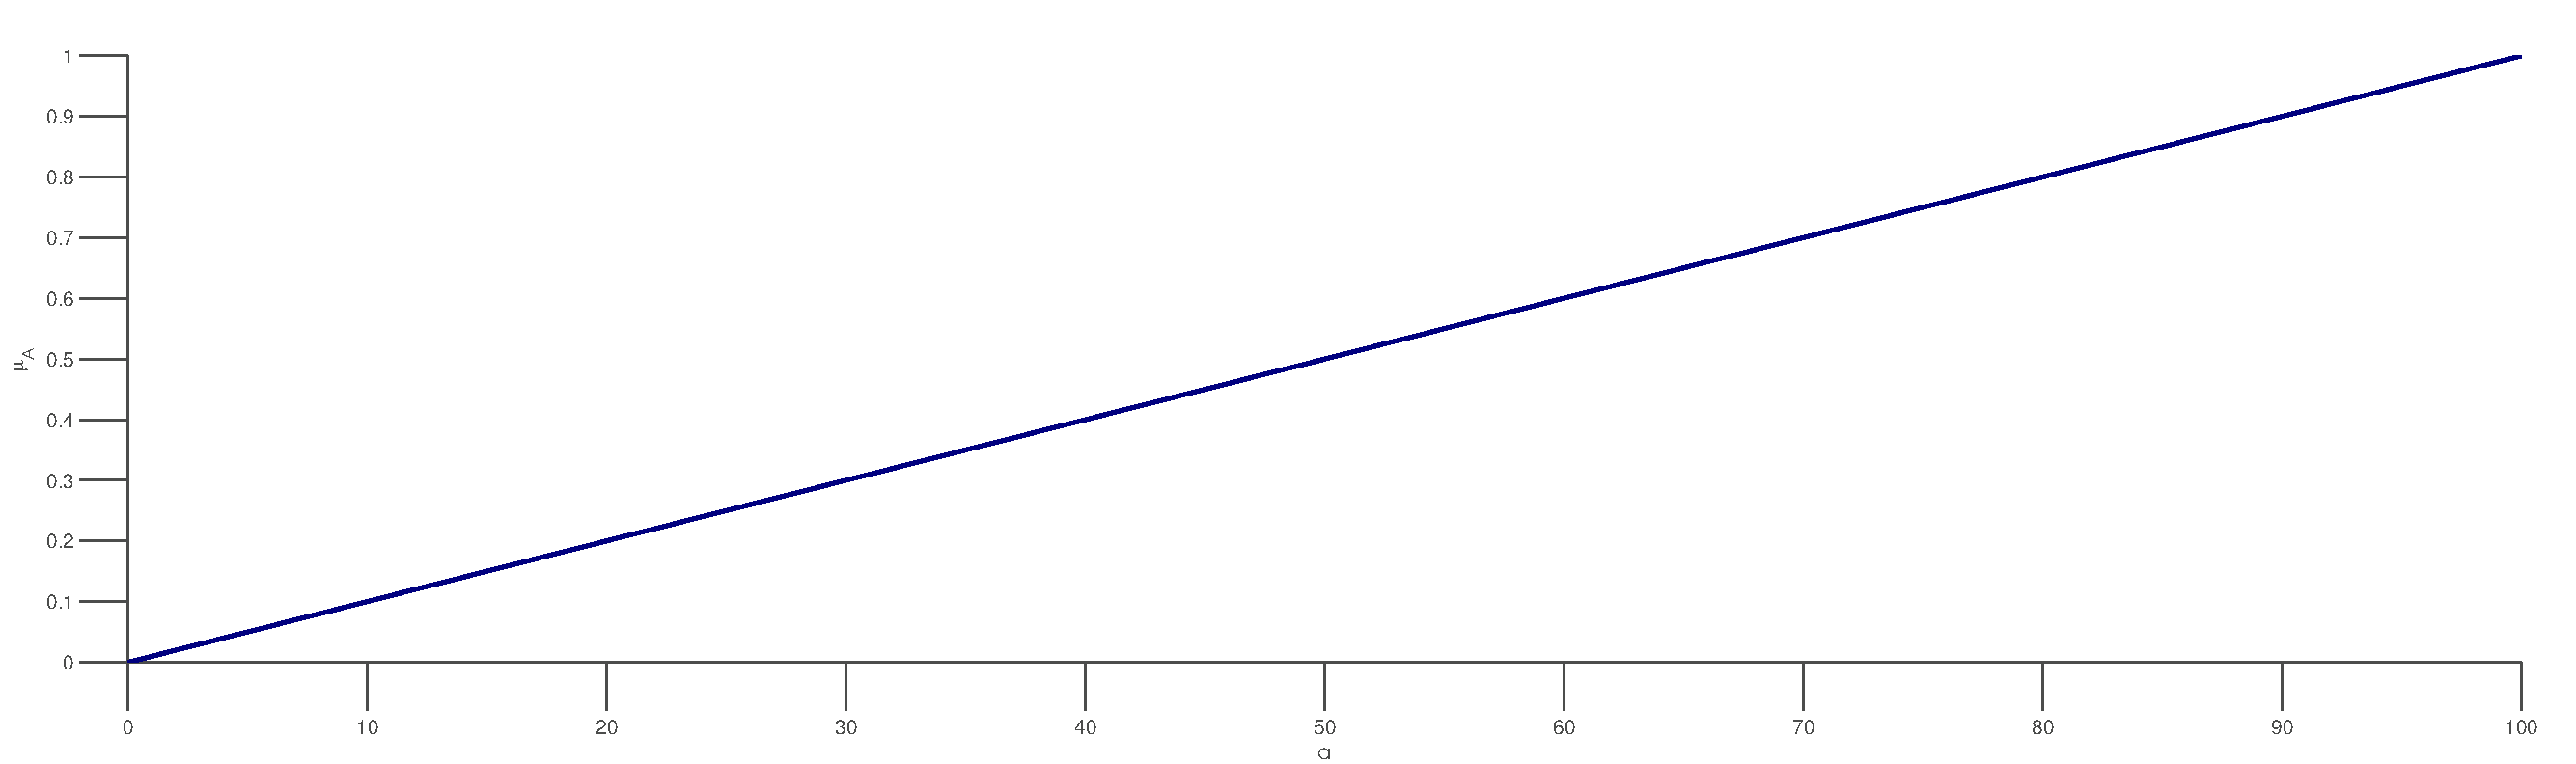
\includegraphics[width=\textwidth]{FMF_ex}
    \caption[Graphical representation of a single FMF]{Fuzzy membership function for $\protect\fuzzyset{A}=\left \{ \text{'Is old'} \right \}$}
    \label{fig:FMF_ex}
\end{figure}
\todo{Increase graphic font}
\begin{figure}[H]
    \centering
    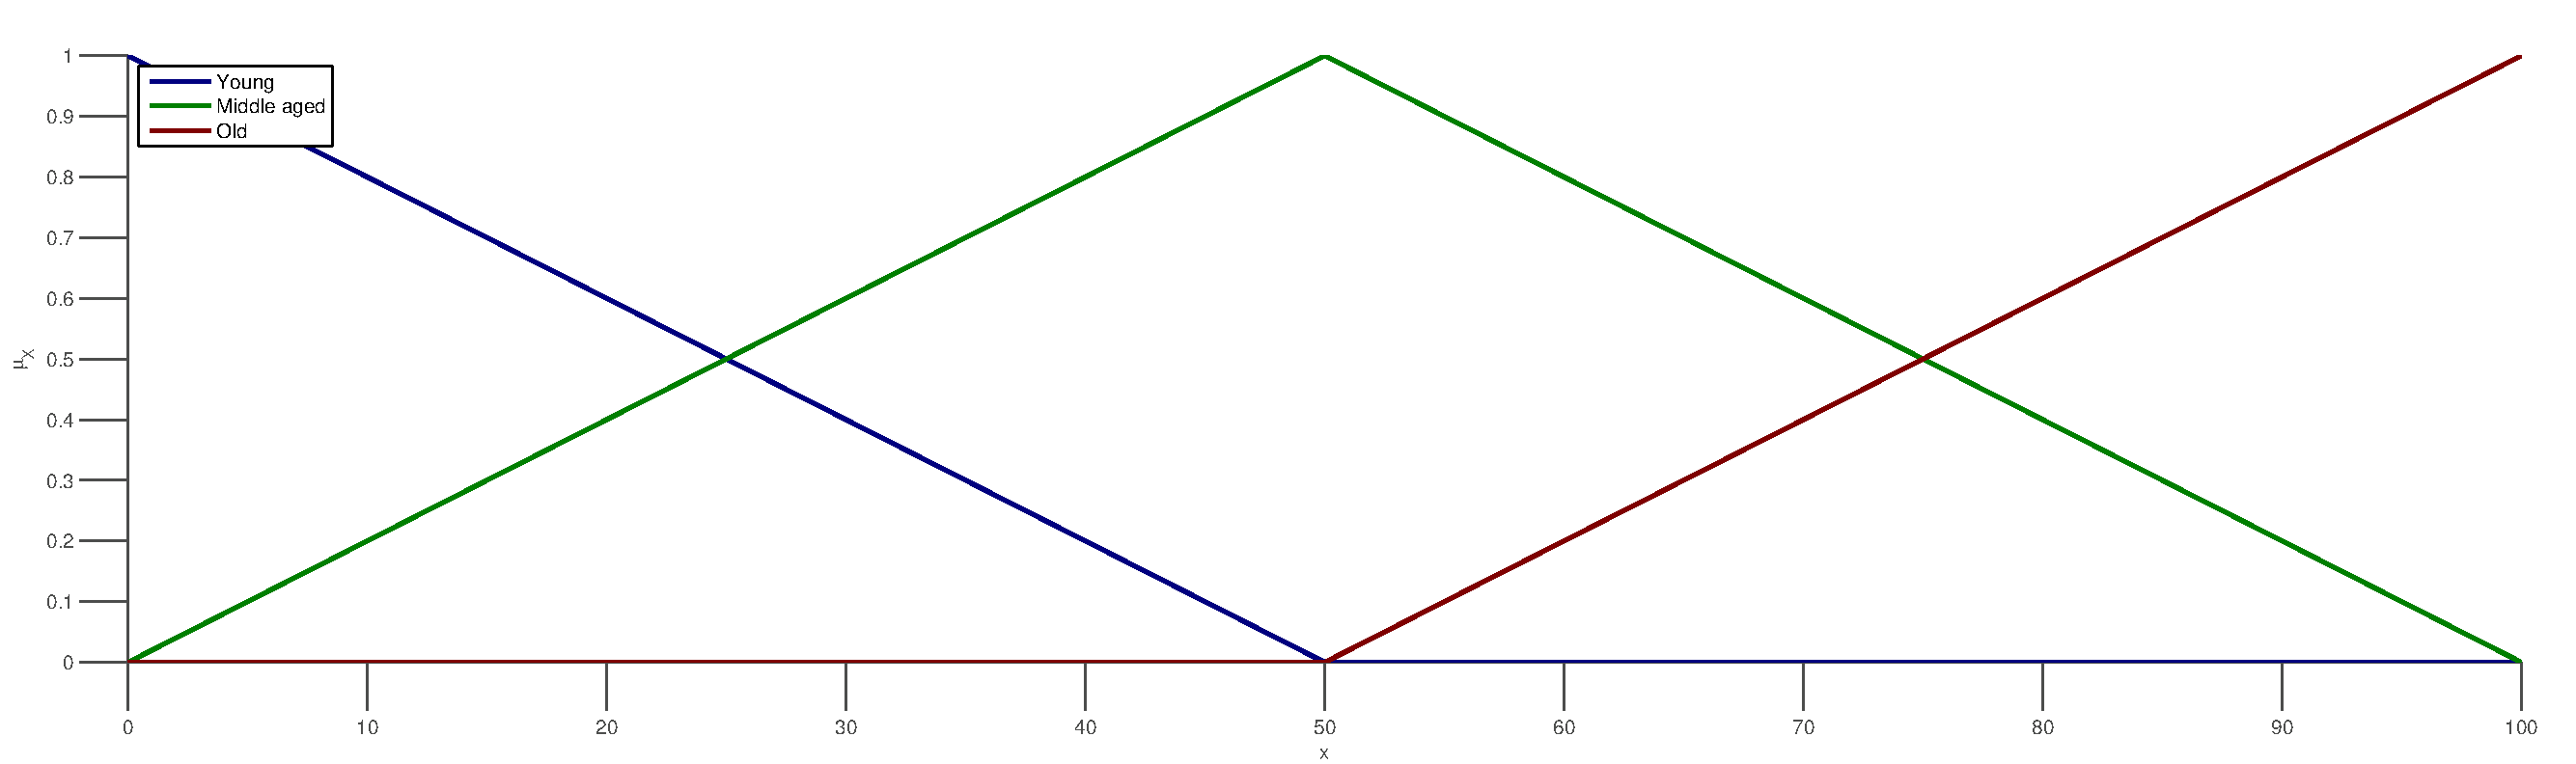
\includegraphics[width=\textwidth]{FMF_ex2}
    \caption[Graphical representation of multiple FMFs]{Fuzzy membership function for $\protect\fuzzyset{A}=\{\text{'Is young'}\}, \protect\fuzzyset{B}=\{\text{'Is middle-aged'\}}\text{ and }\protect\fuzzyset{C}=\{\text{'Is old'}\}$}
    \label{fig:FMF_ex2}
\end{figure}
%------------------------------------------------------------------------------------
\section{Fuzzy logic}
\label{section:fuzzy_logic}
Fuzzy sets and set theory can, in the same manner as classical boolean sets, be used to define logical expressions. Fuzzy logic allows for half-truths, i.e. truth values in the interval [0,1]. Whereas boolean logic is restricted to truth values of one and zero. The truth value T of a fuzzy preposition P is, therefore a mapping from [0,1] to the universe T, as can be seen in \ref{eq:fuzzy-logic-mapping} \cite{ross2009fuzzy}.
\begin{equation}
    T:u\in U\rightarrow (0,1)
    \label{eq:fuzzy-logic-mapping}
\end{equation}
The truth value of proposition P is therefore given by the membership grade $\mu_{\fuzzyset{A}}(x)$ of $x$ in $\fuzzyset{A}$

Many of the same operators and connectives used in classical logic, does also apply to fuzzy logic. This thesis will only present the rules necessary for the scope of the thesis, which are the following \cite{ross2009fuzzy}:\\
\noindent Negation
\begin{equation}
    T(\fuzzyset{\overline{P}})=1-T(\fuzzyset{P})) {}\label{eq:negation}
\end{equation}
Disjunction
\begin{equation}
    \fuzzyset{P}\lor \fuzzyset{Q}:x \text{ is } \fuzzyset{A} \text{ or } \fuzzyset{B}\quad T(\fuzzyset{P} \lor \fuzzyset{Q})=max(T(\fuzzyset{P}),T(\fuzzyset{Q}))\label{eq:disjunction}
\end{equation}
Conjunction
\begin{equation}
    \fuzzyset{P}\land \fuzzyset{Q}:x \text{ is } \fuzzyset{A} \text{ and } \fuzzyset{B}\quad T(\fuzzyset{P} \land \fuzzyset{Q})=min(T(\fuzzyset{P}),T(\fuzzyset{Q}))\label{eq:conjunction}
\end{equation}
Implication
\begin{equation}
    \fuzzyset{P}\to \fuzzyset{Q}: x \text{ is } \fuzzyset{A} \text{, then }x \text{ is } \fuzzyset{B}
    \label{eq:implication}
\end{equation}
\[ T(\fuzzyset{P}\to \fuzzyset{Q})=T(\fuzzyset{\overline{P}}\lor\fuzzyset{Q})=max(T(\fuzzyset{\overline{P}}),T(\fuzzyset{Q}))  \]


\noindent Implication can also be written in rule based form
\[ \fuzzyset{P} \to \fuzzyset{Q} \text{ is,  IF } x \text{ is } \fuzzyset{A} \text{ , THEN } t \text{ is } \fuzzyset{B}\]
\[ \Leftrightarrow \]
\[  R=(\fuzzyset{A}\times\fuzzyset{B})\cup (\overline{\fuzzyset{A}}\times \fuzzyset{Y})\]
\noindent With the membership function:
\begin{equation}
    \mu_{\fuzzyset{R}}(x,y)=max[\mu_{\fuzzyset{A}}(x)\land\mu_{\fuzzyset{B}}(y),(1-\mu_{\fuzzyset{A}}(x))]
    \label{eq:implication-orig}
\end{equation}
Equation \ref{eq:implication-orig} is the fuzzy equivalent to the material implication  $\neg A \lor B$ used in traditional boolean logic\cite{ying2002implication}, where $\neg A = 1-\mu_{\fuzzyset{A}}(x)  $ and $B = \mu_{\fuzzyset{A}}(x)\land\mu_{\fuzzyset{B}}(y)$. However, fuzzy logic has multiple implication operators \cite{ross2009fuzzy}. The work in this thesis will use Mamdani's implication, see equation \ref{eq:mamdani}, since it is the most commonly used one.
\begin{equation}
    \mu_{\fuzzyset{R}}(x,y)=min[\mu_{\fuzzyset{A}}(x),\mu_{\fuzzyset{B}}(x))]
    \label{eq:mamdani}
\end{equation}




%------------------------------------------------------------------------------------
\section{Fuzzy (rule-based) systems}
Fuzzy logic can be used to model complex systems described in natural language, originally written to be interpreted by humans. Such knowledge can often be written as rules in the following form \cite{ross2009fuzzy}.
\begin{equation}
    \text{IF premise (antecedent), THEN conclusion (consequent)}
\end{equation}
Combining multiple rules enables one to describe complex systems in a relatively simple structure. Rules can, furthermore, contain multiple antecedents and consequents. However, this raises the question of how multiple antecedents, as shown in rule \ref{eq:conj-ant}, can be  decomposed into a single antecedent and the rules aggregated into a single consequent \cite{ross2009fuzzy}.
\begin{equation}
    \text {IF $x$ is $\fuzzyset{A_1}$ and $\fuzzyset{A_2}$ \dots and $\fuzzyset{A_L}$ THEN $y$ is $\fuzzyset{B_s}$}
    \label{eq:conj-ant}
\end{equation}
Conjunctive antecedents can be rewritten as a new fuzzy set

\[ \fuzzyset{A_s}=\fuzzyset{A_1}\cap \fuzzyset{A_2} \cap \dots \cap \fuzzyset{A_L} \]
with the membership function
\[ \mu_{\fuzzyset{A_S}}(x)=min \left [\mu_{\fuzzyset{A_1}}(x),\mu_{\fuzzyset{A_2}}(x),\dots,\mu_{\fuzzyset{A_3}}(x) \right ] \]
Rule \ref{eq:conj-ant} can then be rewritten as
\[ \text{IF $\fuzzyset{A_S}$ THEN $\fuzzyset{B_S}$} \]
Disjunctive antecedents can similarly be written as
\[ \fuzzyset{A_s}=\fuzzyset{A_1}\cup \fuzzyset{A_2} \cup \dots \cup \fuzzyset{A_L} \]
\[ \mu_{\fuzzyset{A_S}}(x)=max \left [\mu_{\fuzzyset{A_1}}(x),\mu_{\fuzzyset{A_2}}(x),\dots,\mu_{\fuzzyset{A_3}}(x) \right ] \]
The same principle can be applied to find the overall consequent when multiple rules apply. Conjunctive rules where both consequents must be applied can be found by  the fuzzy intersection of all the rule consequents. Whereas disjunctive rules use the fuzzy union of the rule consequents.



\section{A fuzzy logic model for COLREGs}
\label{section:model}
\todo{Move section to Impl?}
Antecedents consequents and rules are needed in order to make a fuzzy system for a COLREGs compliant auto pilot. The model used in this thesis is created by \textcite{perera2012intelligent} and has four antecedents, two consequents and an extensive rule set of nearly 200 rules. The antecedents used are: relative bearing to the target vessel, relative course of the target vessel, distance between the vessels, and the ratio between the vessels speed. The main vessels relative bearings are divided into ten sets. These resulting sectors represent the different sets in the relative course universe [0, 360]. The relative courses of the target vessel are ,likewise, divided into eight sectors, which represent sets in the relative course universe [0, 360]. The distance universe consist of three sets, representing radii from the main vessel, called $R_A, R_B$ and $R_{VD}$. $R_{VD}$ is the vessel domain into which other vessel shall not enter. $R_A$ and $R_B $depicts the area around the main vessel in which other vessels are detected. $R_A$ when the main vessel is the give way vessel and $R_B$ when it is the stand on vessel. A graphical representation of the bearing, range and course sectors can be seen in figure \ref{fig:model}. The final antecedent, $\text{speed ratio} =\frac{V_{target}}{V{main}}$, consist of three sets: $<1, \approx1 \text{ and } >1$.
Visualizations of the antecedent FMFs, as well as their distribution in their corresponding universes, can be seen in figure \ref{fig:antecedent_fmfs}.

Finally a rules set is needed to connect the antecedents with the consequents. The rule set used for this thesis is based on  the rules, seen in table \ref{tab:rules} developed by \textcite{perera2012intelligent}. A few rules have furthermore been added to handle overtake scenarios. These can be seen in table \ref{tab:rules_own}
\todo{Explain tables?}

An analysis and optimization of the values used to specify the FMFs and the rules in the rule set are unfortunately outside of the scope for this thesis. The values are therefore used as specified in previous research \cite{perera2012intelligent}, with the exception of a few added rules to ensure collisions avoidance when one vessel is overtaking another.


\begin{figure}[H]
    \centering
    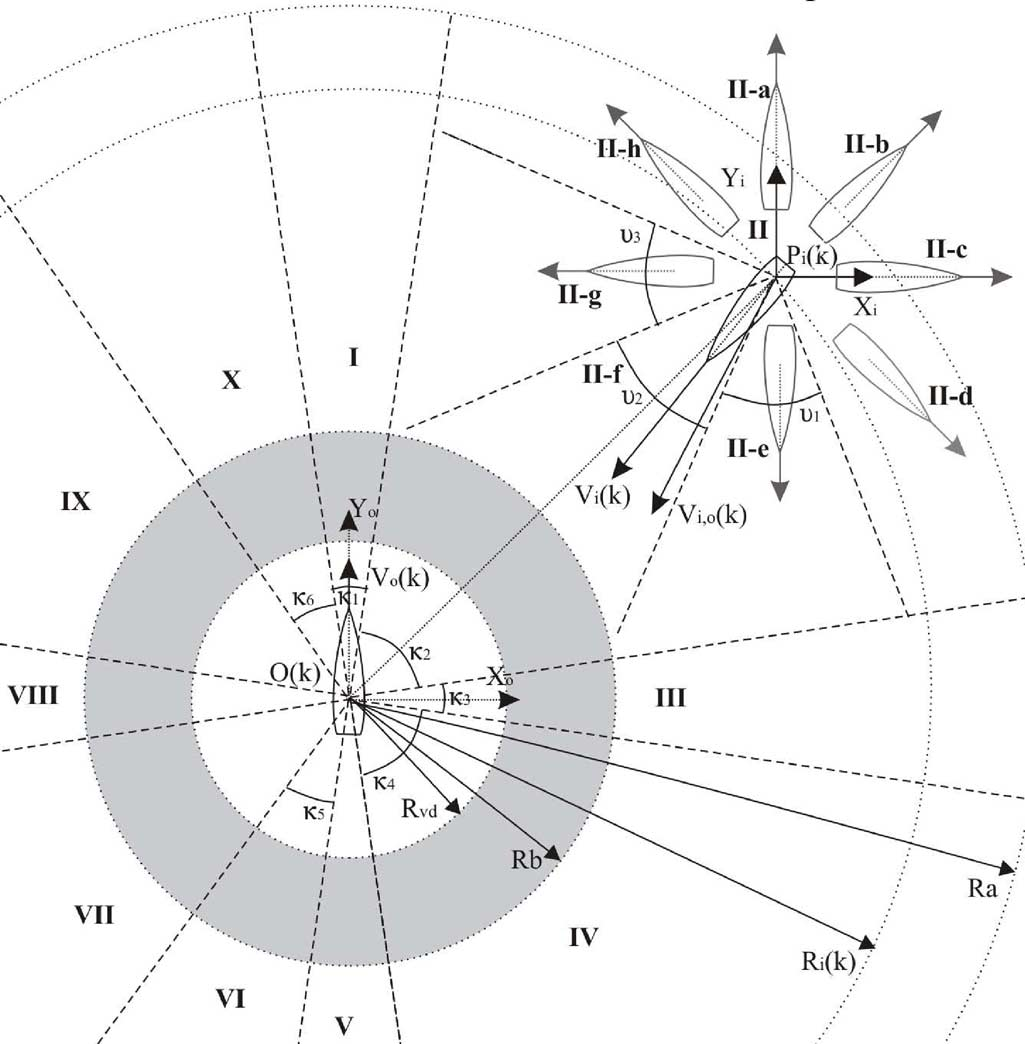
\includegraphics[width=\linewidth]{Figures/model}
    \caption{Mathematical representation of the inputs to a FIS for a two vessel collision situation\cite{perera2012intelligent}}
    \label{fig:model}
\end{figure}

\begin{figure}[H]
    \begin{tabular}{cc}

        \subfloat[Relative bearing of the target vessel from the main vessel]{
            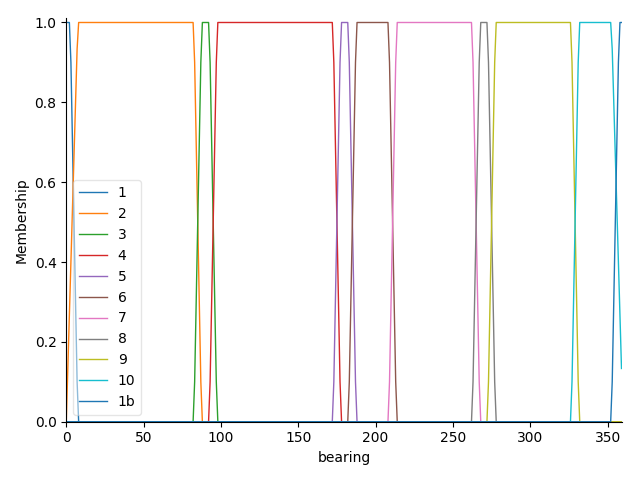
\includegraphics[width=.49\linewidth]{Figures/FMF_bearing}
        } &
        \subfloat[Relative course of the target vessel to the main vessel]{
            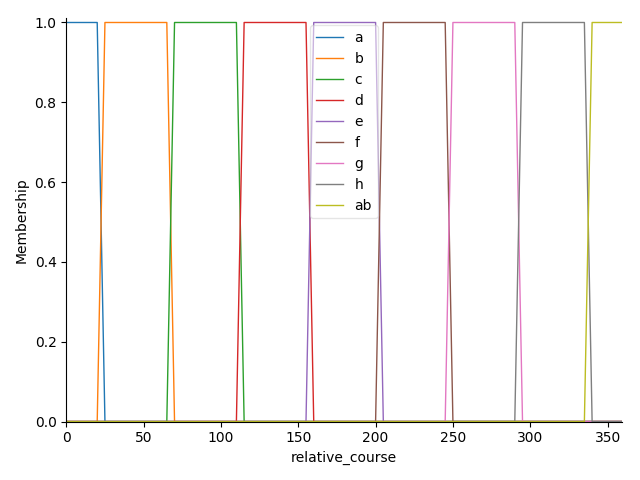
\includegraphics[width=.49\linewidth]{Figures/FMF_rel_course}
        }   \\
        \subfloat[Speed ratio target vessel/main vessel]{
            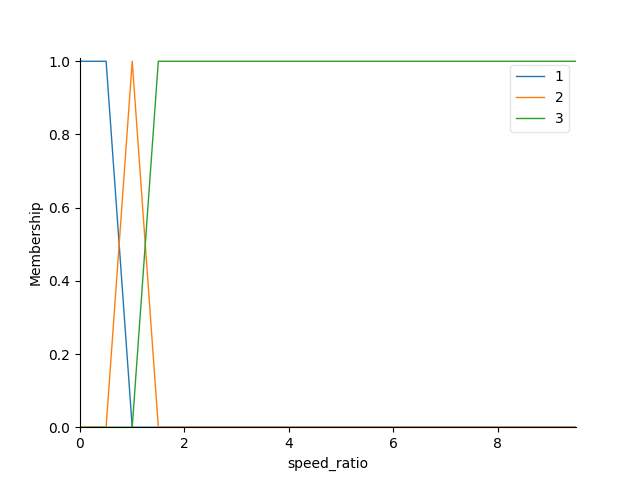
\includegraphics[width=.49\linewidth]{Figures/FMF_speed_ratio}
        } &
        \subfloat[Distance between the main vessel and the target vessel]{
            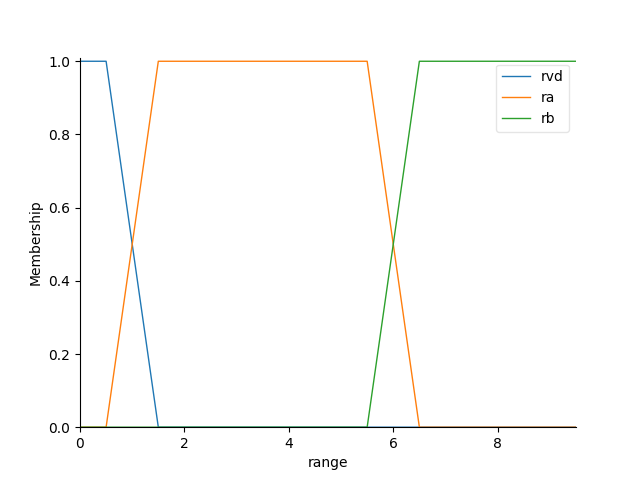
\includegraphics[width=.49\linewidth]{Figures/FMF_range}
        }
    \end{tabular}

    \caption{Antecedent FMFs}
    \label{fig:antecedent_fmfs}
\end{figure}



\begin{figure}[H]

    \begin{tabular}{cc}

        \subfloat[Course change of the main vessel]{
            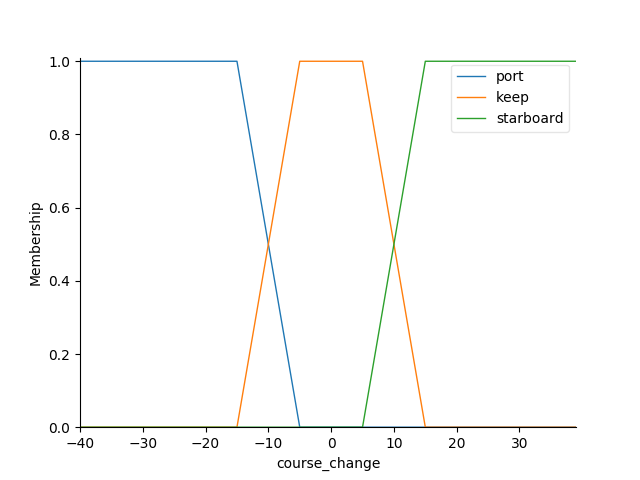
\includegraphics[width=.45\linewidth]{Figures/FMF_course_change}
        } &
        \subfloat[Speed change of the main vessel]{
            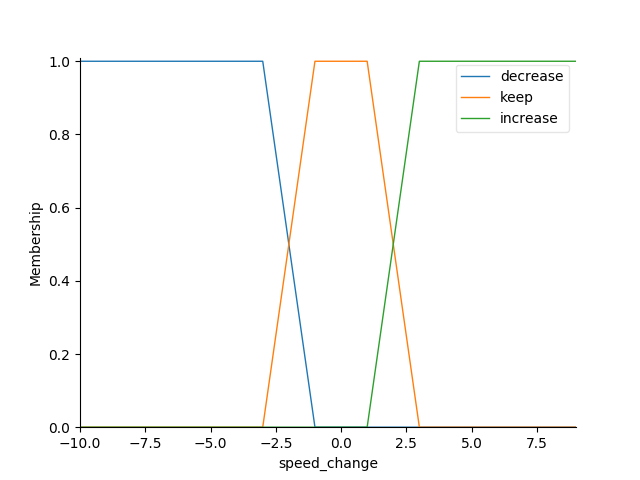
\includegraphics[width=.45\linewidth]{Figures/FMF_speed_change}
        }
    \end{tabular}
    \caption{Consequent FMFs}
    \label{fig:consequent_fmfs}
\end{figure}





\section{Mamdani's fuzzy inference method}
\label{section:FIS}
This thesis will, as mentioned in section \ref{section:fuzzy_logic}, use the Mamdani implication operator in its Fuzzy Inference System (FIS). Mamdani's method was chosen since it is the most common one in practice literature \cite{ross2009fuzzy}.


The following subsections will explain Mamdani's method by going through an example based on the model presented in section \ref{section:model}. The example uses a scenario where two vessels are located in a 2 dimensional 10*10 NM Cartesian coordinate system.\\
Vessel A starts at coordinate (0; -4,5) with heading 0, speed 5 kts and rate of turn 2 degrees per second.\\
Vessel A starts at coordinate (-4,5; -4,5) with heading 203, speed 10 kts and rate of turn 2 degrees per second.
The initial state of the scenario is depicted in figure \ref{fig:scenario_1a}
\begin{figure}[H]
    \centering
    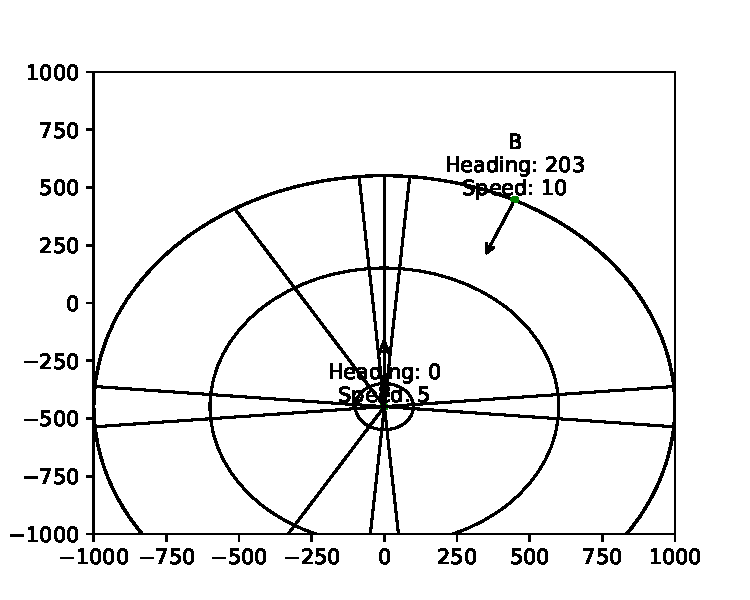
\includegraphics[width=\textwidth]{Figures/scenario_1a}
    \caption{Initial state of the example scenario}
    \label{fig:scenario_1a}
\end{figure}


A FIS can be said to consist of six steps \cite{fis_princeston}:
\begin{enumerate}
    \item Rule determination
    \item Input fuzzification
    \item Combination of antecedents
    \item Obtain consequences
    \item Aggregate consequences
    \item Defuzzification
\end{enumerate}

This example will use a subset of the rules used in the real system.
The rules used are:
\begin{enumerate}[label=\textbf{Rule \arabic*},ref=Rule \arabic*]
    \item \label{rule:1} IF target in sector II AND relative course is in sector f  AND speed ratio is greater than 1  AND range is $R_vd$ OR $R_b$ OR $R_a$ \\THEN change course to starboard  AND  reduce speed.
    \item IF target in sector II AND relative course is in sector e AND  speed ratio is greater than 1  AND  range is $R_vd$ OR $R_b$ OR $R_a$ \\THEN change course to starboard  AND  reduce speed.
\end{enumerate}

Next the crisp values, gained when applying the model presented in section \ref{section:model} on the scenario in figure \ref{fig:scenario_1a}, are fuzzified. The target vessel is located in sector II with a relative bearing of 26,7\textdegree, which results in a membership value of 1 in sector 2 as shown by the red line in figure \ref{fig:FMF_bearing_fuzzified}

The same principle is applied to the three other inputs: relativist course, distance, and speed ratio. Distance and speed ratio will also, in this case, yield membership values of 1, for the fuzzy sets distance $R_a$ and speed ratio>1 . However, the relative course of 203 is located in the fuzzy area between sector 2-e and 2-f which results in membership values of 0,4 and 0,6 respectively, as shown in figure \ref{fig:FMF_rel_course_fuzzified}.
\begin{figure}[H]

    \begin{tabular}{cc}

        \subfloat[Bearing antecedent]{
            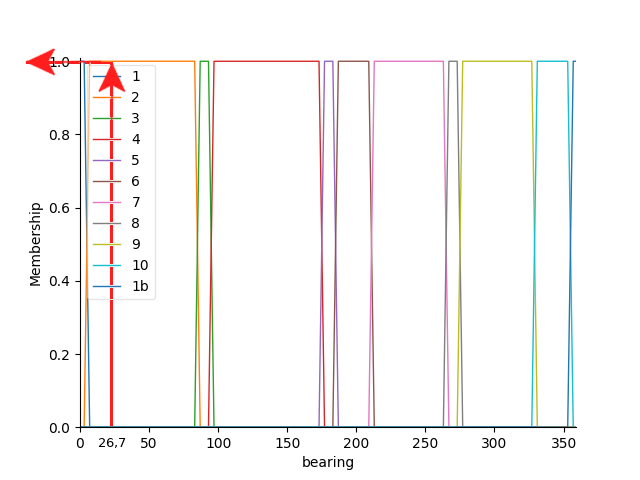
\includegraphics[width=.45\linewidth]{Figures/FMF_bearing_fuzzified}
            \label{fig:FMF_bearing_fuzzified}
        } &
        \subfloat[Relative course antecedent]{
            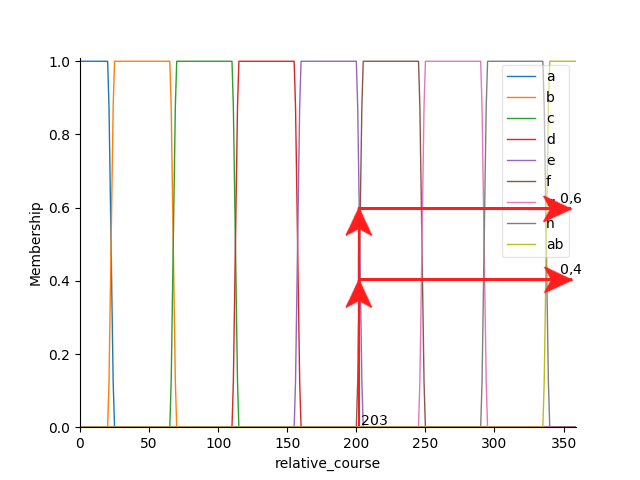
\includegraphics[width=.45\linewidth]{Figures/FMF_rel_course_fuzzified}
            \label{fig:FMF_rel_course_fuzzified}
        }
    \end{tabular}
    \caption{Fuzzified antecedent FMFs for the example scenario}
\end{figure}

The membership values gained for the individual antecedents can then be combined using the AND and OR operators specified in the rule set. This results in the following calculations.
\begin{equation}
    Rule 1: min(1; 0,6; 1; max(0;0;1))=0,6
    \label{eq:ant_comb_rule_1}
\end{equation}
\begin{equation}
    Rule 2: min(1; 0,4; 1; max(0;0;1))=0,4
    \label{eq:ant_comb_rule_2}
\end{equation}

Mamdani's inference method is then used on each rule to obtain the consequent value. This is done by taking the minimum of the antecedent value from the previous step and the consequent. The result is a clipped consequent FMF, as seen in figures \ref{fig:ex_cons_1} and \ref{fig:ex_cons_2}


\begin{figure}[H]

    \begin{tabular}{cc}

        \subfloat[Course change of the main vessel]{
            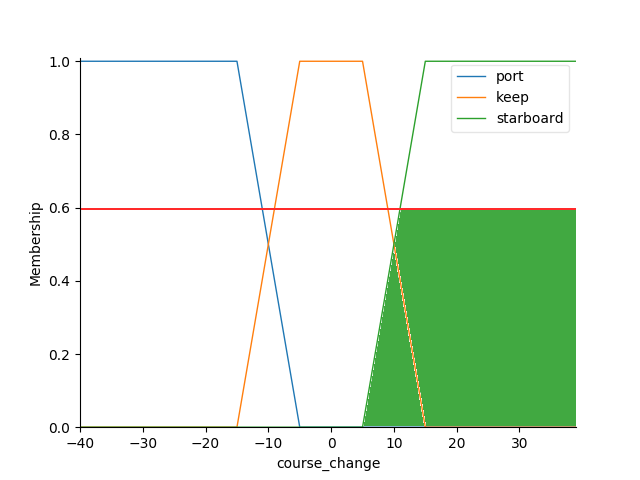
\includegraphics[width=.45\linewidth]{Figures/FMF_course_change_conseq_ex_06}
        } &
        \subfloat[Speed change of the main vessel]{
            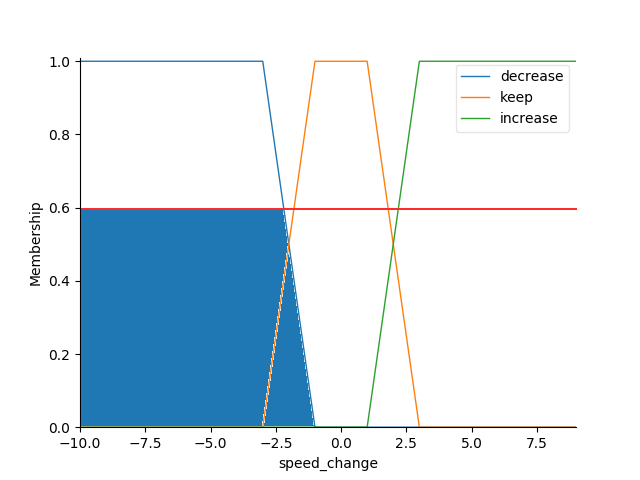
\includegraphics[width=.45\linewidth]{Figures/FMF_speed_change_conseq_ex_06}
        }
    \end{tabular}
    \caption{Consequent FMFs for rule 1 after applying Mamdani's inference method }
    \label{fig:ex_cons_1}
\end{figure}


\begin{figure}[H]

    \begin{tabular}{cc}

        \subfloat[Course change of the main vessel]{
            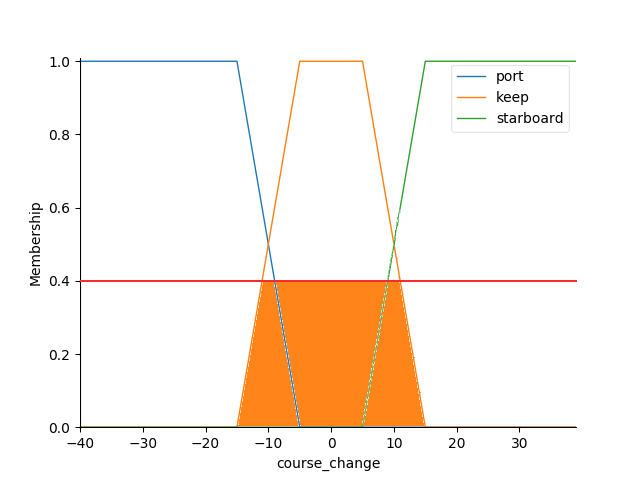
\includegraphics[width=.45\linewidth]{Figures/FMF_course_change_conseq_ex_04}
        } &
        \subfloat[Speed change of the main vessel]{
            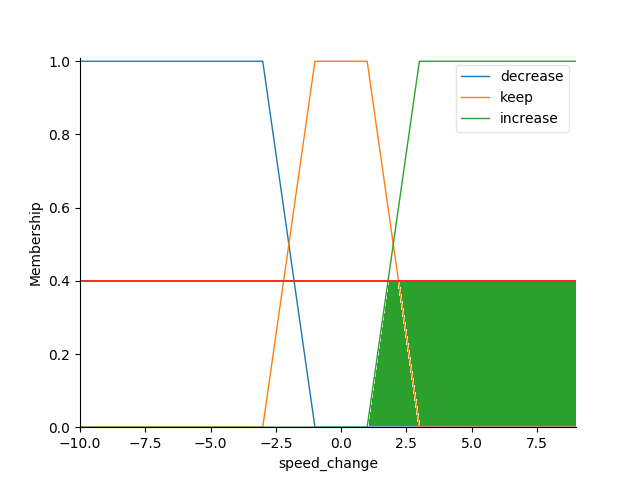
\includegraphics[width=.45\linewidth]{Figures/FMF_speed_change_conseq_ex_04}
        }
    \end{tabular}

    \caption{Consequent FMFs for rule 2 after applying Mamdani's inference method }
    \label{fig:ex_cons_2}
\end{figure}

The clipped consequents, one for each rule, must then be combined. This is achieved by taking the maximum of each consequent, to create a combined FMF. The result is presented in figure \ref{fig:ex_cons_tot}

\begin{figure}[H]

    \begin{tabular}{cc}

        \subfloat[Course change of the main vessel]{
            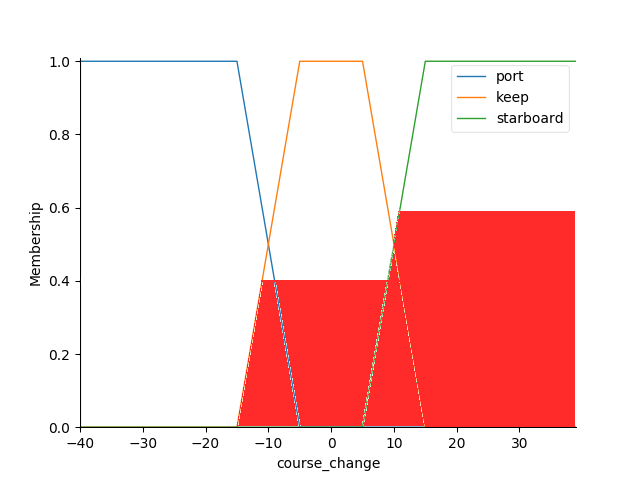
\includegraphics[width=.45\linewidth]{Figures/FMF_course_change_conseq_ex_tot}
        } &
        \subfloat[Speed change of the main vessel]{
            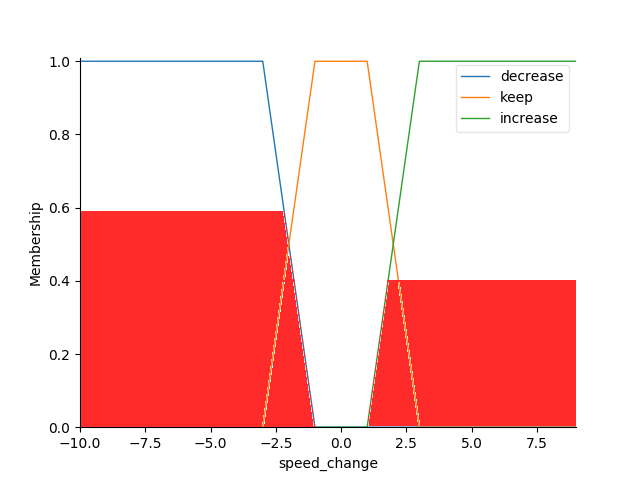
\includegraphics[width=.45\linewidth]{Figures/FMF_speed_change_conseq_ex_tot}
        }
    \end{tabular}

    \caption{Combined Consequent FMFs for the example scenario}
    \label{fig:ex_cons_tot}
\end{figure}

Finally the fuzzy sets gained from the previous step need to be converted into a crisp numerical value that can be used by the auto pilot. This process is called defuzzification and is in this case achieved by calculating the centroid value of FMFs in figure \ref{fig:ex_cons_tot}. The results are a +15.5\textdegree course change and a -1,7 knot speed change.
%!TEX root = ../main.tex
% !TeX spellcheck = en_GB 


\chapter{Implementation}
\label{chap_impl}
The objective of this thesis was to implement and evaluate a  collision avoidance  algorithm for USVs. Several related approaches where analysed before the fuzzy logic approach presented by \textcite{perera2012intelligent}, was chosen to be implemented.
The solution presented in the original paper is implemented in MATLAB, while the solution presented here is implemented in Python. Python was chosen due to the writer's previous knowledge of the language as well as the availability of fuzzy logic python libraries. The library used in this implementation is called SciKit-Fuzzy \cite{josh_warner_2017_1002946}.

\section{The fuzzy inference system}
Scikit fuzzy provides a simple application programming interface to setup a FIS. This section will describe the process setting up a simple FIS that calculates salary based on age and the number of previous jobs. Fuzzy sets for age are set up int the same way as in \ref{sec:fuzzy_sets}, but with age ranges more appropriate for the example. The sets are therefore young = 18 - 35, middle aged = 30 - 50, and old 45-65.  Additionally, job and salary sets are introduced. Line 4-6 in listing \ref{listing:fis} initializes the universes for the different fuzzy sets. These are 18-100 for age and 0-10 for jobs, both with a step of 1. Age and jobs act as antecedents in the FIS and the initialization call is therefore to  \texttt{ctrl.Antecedent} Salary goes from 1500-10000 with steps of 500 and acts as consequent and is therefore initialized with  \textit{ctrl.Consequent}. The numbers used are made up for the sake of the example.

Next, the membership functions are initialized in lines 7-15. The age sets are defined  on lines 7-9 as described above.
Three different job sets are defined: \textit{few} (<3),  \textit{medium} (2-6), and \textit{many} (>5). The salary sets are \textit{low} (1500 - 2500),  \textit{medium} (2000-7000), and \textit{high} (<6000). All sets are initialized using \texttt{fuzz.trimf} which produces a triangular membership function. The resulting FMFs are visualized in figure \ref{fig:fmf_ex3}
\begin{figure}[H]
    \begin{tabular}{cc}

        \subfloat[Age antecedent]{
            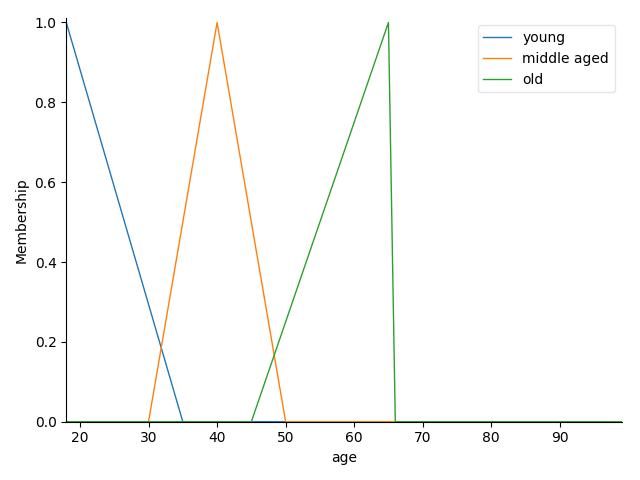
\includegraphics[width=0.5\textwidth,height=0.42\textheight,keepaspectratio]{Figures/age_ex}
            \label{fig:age_ex}
        } &
        \subfloat[Jobs antecedent]{
            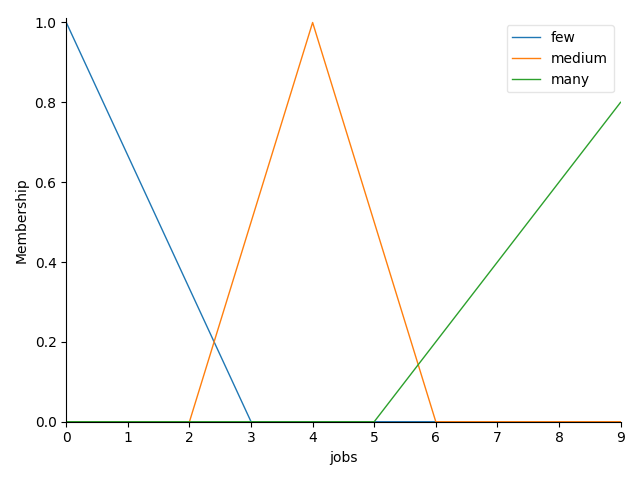
\includegraphics[width=.49\linewidth,height=0.42\textheight,keepaspectratio]{Figures/jobs_ex}
            \label{fig:jobs_ex}
        }   \\
        \multicolumn{2}{c}{\subfloat[Salary consequent]{
                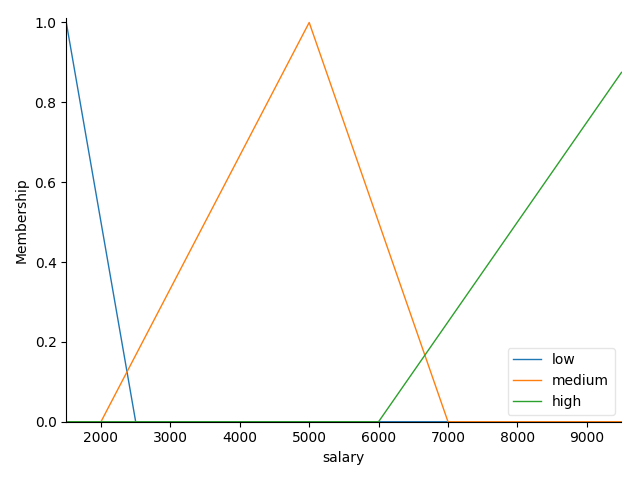
\includegraphics[width=\linewidth,height=0.42\textheight,keepaspectratio]{Figures/salary_ex}
                \label{fig:salary_ex}
            }}
    \end{tabular}

    \caption{FMSs used in example FIS}
    \label{fig:fmf_ex3}
\end{figure}

Next, the following rules are defined, on lines 16 -21, to connect the antecedents with the consequents:

\begin{enumerate}[label=\textbf{Rule \arabic*},ref=Rule \arabic*]
    \item IF young  OR few jobs THEN salary is low
    \item IF middle-aged  AND few jobs THEN salary is low
    \item IF middle-aged  OR medium amount of  jobs THEN salary is medium
    \item IF middle-aged  AND many jobs THEN salary is high
    \item IF old  OR many jobs THEN salary is high
\end{enumerate}

Finally, the rules are passed to the Control System on line 25  and  \\ \texttt{ctrl.ControlSystemSimulation} is called to complete the FIS initialization.
The system is now ready to take input and calculate output based on the rule set specified. An example using age = 35 and jobs = 1 is input on lines 25-28 and the output printed on lines 30-32. The example outputs a salary of 4157.





\begin{listing}[H]
    \inputminted[linenos, breaklines=true,fontsize=\scriptsize, numberblanklines=false]{python}{../src/example.py}
    \caption{FIS initialization}
    \label{listing:fis}
\end{listing}

\section{Architecture}
This section will present the high-level structure of the implementation with the help of the class diagram seen in figure \ref{fig:class_diagram}. Each class and their interactions will be briefly presented.
\begin{figure}[H]
    \centering
    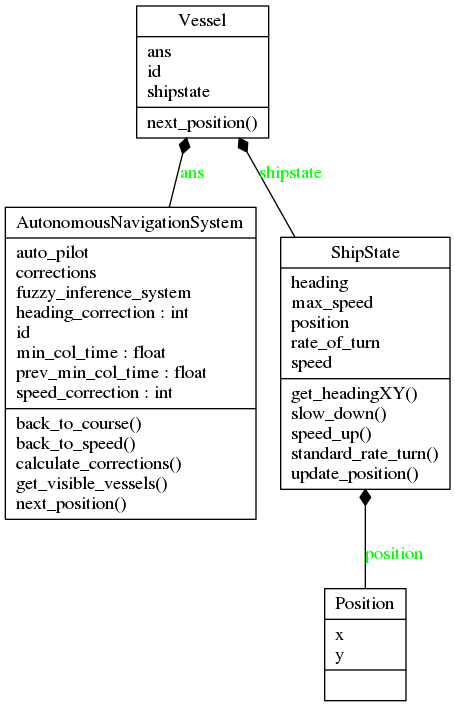
\includegraphics[width=\textwidth,height=0.75\textheight,keepaspectratio]{../src/classes_Pyreverse}
    \caption{Class diagram}
    \label{fig:class_diagram}
\end{figure}
\subsection{Classes}
Each simulation scenario consists of at least one vessel. These vessels are represented by the \textit{Vessel} class. The current state of the vessel is represented by the \textit{ShipState} class which also contains the \textit{Position} class. Furthermore, each vessel needs a navigation system, which is represented by the \textit{AutonomousNavigationSystem} class. The classes will be more thoroughly presented in the following subsections.
\subsubsection{Vessel}
\textit{Vessel} is the main class and the class with which the simulation script interacts.
It contains, apart from the previously mentioned \textit{AutonomousNavigationSystem} and \textit{ShipState} an id and a method to calculate its position in the next time frame.
A new vessel object is created with the following call:
\begin{minted}{python}
Vessel(id, heading, position_x, position_y, speed, max_speed, 
    rate_of_turn, fuzzy_inference_system, auto_pilot)
\end{minted}
This constructor call specifies the ID for the vessel as well as its initial position, speed and heading. Furthermore, it defines the vessels maximum speed and rate of turn. The two final parameters specify the fuzzy inference system to use and whether the vessel shall use the navigation system. Setting the final boolean to false creates a rogue vessel that will just keep its initial speed and heading, thereby not complying with the COLREG rules. The \textit{Vessel} class has only one method, which calculates the vessels position in the next time frame after applying possible corrections to heading and speed.
\subsubsection{Position}
The position class simply holds the vessels current coordinates in the Cartesian coordinate system used.
\subsubsection{ShipState}
ShipState holds information about the state of the vessel in the current time frame. This includes the vessels current position, heading and speed. The simulation does not distinguish between course and heading since no drift is simulated.
Furthermore, limits such as maximum allowed speed and standard rate of turn are specified in this class. Finally, the class holds methods to change the ships heading by the specified standard rate of turn or speed by 1 kt, for the next time frame.


\subsubsection{AutonomousNavigationSystem}
\label{sec:ANS}
The AutonomousNavigationSystem class from now on referred to as ANS is what separates an autonomous vessel from an ordinary vessel. The ANS combines the information from the ShipState class with situational awareness information provided by a separate Situational Awareness (SA) module, in order to calculate needed corrections to speed and course.

The SA is in this simulation case represented by a service that holds all information regarding the current scenario. A real system would have a SA module that reads and processes information from different sensors, such as LiDAR, cameras, on board the vessel. Information needed about a target vessel is its heading, speed, and position. These are used to calculate the four different inputs to the FIS system. Listing \ref{listing:rel_bear_calc} shows the method used to calculate the relative bearing fed into the FIS system. Compass bearing is first calculated from the two provided coordinate pairs after which the result is converted into a relative bearing. Relative course is then calculated as the observed vessels heading - the own vessels heading, as shown in listing \ref{listing:rel_course_calc}. Distance can be obtained by using the Pythagorean theorem on the differences between the vessels in the X and Y axis. Finally, speed ratio is defined as $\frac{\text{Speed of the observed vessel}}{\text{Speed of the own vessel}}$.
\begin{listing}

    \begin{minted}[linenos, breaklines=true,fontsize=\scriptsize, numberblanklines=false]{python}
rel_course = observed_vessel.shipstate.heading - shipstate.heading
if rel_course < 0:
    rel_course = 360 + rel_course
    \end{minted}
    \caption{Relative course calculation}
    \label{listing:rel_course_calc}
\end{listing}

These inputs are fed into the FIS system, for each target vessels, and the recommended corrections presented by FIS are stored in an array. The expected time until collision for each target vessel is also calculated. Knowing the distance between the vessels, their relative velocity is needed to calculate the time. Equation \ref{eq:rel_vel_calc} shows the relative velocity calculation, based on the law of Cosines. \textit{V} stands for velocity, $\theta$ for heading, the subscript \textit{m} for own vessel and \textit{t} for target vessel.

\begin{equation}
    V_r=\sqrt{V_m^2 + V_t^2-2  V_mV_tcos(\theta_m-\theta_t)}
    \label{eq:rel_vel_calc}
\end{equation}

The previous calculations result in speed and heading correction suggestions, as well as an expected time until collision, for each target vessel. However, these recommendations might contradict each other and a way to prioritize the corrections in order of urgency is therefore needed. This is in this implementation solved in a simple matter by calculating the weighted arithmetic mean of the corrections using the expected time until collision as weight. The resulting corrections are then stored in ShipState as target heading.

Finally the heading and speed of the vessel is updated in the following manner. The vessels is steered towards the proposed heading change by a maximum of the vessels defined maximum rate of turn. The speed is similarly changed towards the proposed speed by a maximum of one knot. No proposed correction by the FIS means that the vessel is currently not in a scenario that satisfies a rule in the rule set. However, a previous correction suggestion might still not be completed due to the vessels limited rate of turn, acceleration or deceleration.  The vessel will ,therefore, continue to change its heading and speed towards the saved target speed until they are the same.  The target heading is then gradually changed towards the original heading until the vessel is back on its original heading. The process is visualized in Figure \ref{fig:flow_chart}.
\begin{figure}[H]
    \centering
    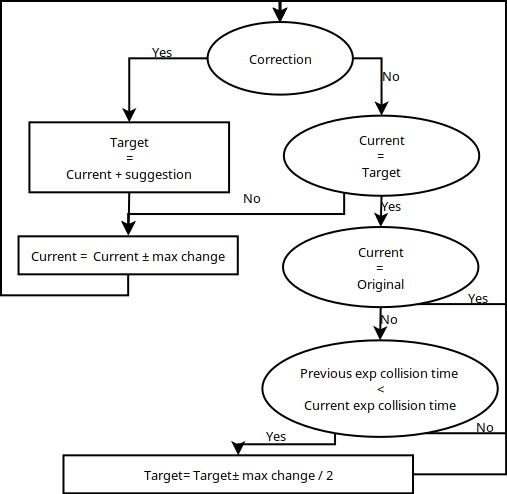
\includegraphics[width=\textwidth,height=0.75\textheight,keepaspectratio]{Figures/flow.png}
    \caption{Flow chart explaining application of heading and speed corrections}
    \label{fig:flow_chart}
\end{figure}

\section{Simulation}
The goal of the implementation is to  simulate a real-world situation with respect to time, speed, acceleration, and rate of turn while neglecting  environmental factors such as weather.
The simulation is therefore limited to two dimensions in a Cartesian coordinate system.
The interval between time frames in the simulation is set to correspond to one second in the real world.
Each iteration of the main simulation loop must, therefore, update the vessels SA by scanning the environment for target vessels. The information gained is then passed to the FIS which generates the course and speed corrections used to update heading and speed as explained in section \ref{sec:ANS}.

The efficiency and quality of the output of the FIS system, is to a large degree dependent on the FMFs. Designing correct FMF and rules to use in a FIS is an extensive mathematical project on its own. The FMFs used in this thesis are, therefore, based on parameters  previously developed by \textcite{perera2010smooth_param}. All FMFs are in the form of isosceles trapezoids, i.e. trapezoids with legs of equal length. The values used is represented in the tables in \ref{tab:fmfs}. The values in the tables from and to columns represent the x values for the midpoint of the trapezoid legs. The fuzziness of the FMF is then defined as the range of the projection of the leg on the x axis. The fuzziness for the FMFs are 5\textdegree for relative bearing and course as well as course change; 0.3NM for range ; 0.5 kts for speed ratio and 1 kts for speed change.

\begin{table}[h!]
    \caption{Parameters for the FMFs used}
    \label{tab:fmfs}
    \begin{minipage}{.5\linewidth}
        \caption{Relative bearing FMF intervals}
        \centering
        \begin{tabular}{ccc}
            \toprule
            Identifier               & from [\textdegree] & to [\textdegree] \\
            \midrule
            \rowcolor{black!20} I    & 355                & 5                \\
            II                       & 5                  & 85               \\
            \rowcolor{black!20}  III & 85                 & 95               \\
            IV                       & 95                 & 175              \\
            \rowcolor{black!20}  V   & 175                & 185              \\
            VI                       & 185                & 211              \\
            \rowcolor{black!20}  VII & 211                & 265              \\
            VIII                     & 265                & 275              \\
            \rowcolor{black!20}  XI  & 275                & 329              \\
            X                        & 329                & 355              \\
            \bottomrule
        \end{tabular}

    \end{minipage}%
    \begin{minipage}{.5\linewidth}
        \caption{Relative course FMF intervals}
        \centering
        \begin{tabular}{ccc}
            \toprule
            Identifier             & from [\textdegree] & to [\textdegree] \\
            \midrule
            \rowcolor{black!20} a  & 337.5              & 22.5             \\
            b                      & 22.5               & 67.5             \\
            \rowcolor{black!20}  c & 67.5               & 112.5            \\
            d                      & 112.5              & 157.5            \\
            \rowcolor{black!20}  e & 157.5              & 202.5            \\
            f                      & 202.5              & 247.5            \\
            \rowcolor{black!20}  g & 247.5              & 292.5            \\
            h                      & 292.5              & 337.5            \\
            \bottomrule
        \end{tabular}

    \end{minipage}%

    \vspace{1em}

    \begin{minipage}{.5\linewidth}
        \caption{Range FMF intervals}
        \centering
        \begin{tabular}{ccc}
            \toprule
            Identifier                   & from [NM] & to [NM] \\
            \midrule
            \rowcolor{black!20} $R_{VD}$ & 0         & 1       \\
            $R_B$                        & 1         & 4       \\
            \rowcolor{black!20} $R_A$    & 4         & 10      \\
            \bottomrule
        \end{tabular}

    \end{minipage}%
    \begin{minipage}{.5\linewidth}
        \caption{Speed factor FMF intervals}
        \centering
        \begin{tabular}{ccc}
            \toprule
            Identifier                 & from & to  \\
            \midrule
            \rowcolor{black!20} $< 1$  & 0    & 0.8 \\
            $\approx 1 $               & 0.8  & 1.2 \\
            \rowcolor{black!20}  $> 1$ & 1.2  & 5   \\

            \bottomrule
        \end{tabular}

    \end{minipage}%
    \vspace{1em}

    \begin{minipage}{.5\linewidth}
        \caption{Course change FMF intervals}
        \centering
        \begin{tabular}{ccc}
            \toprule
            Identifier                     & from [\textdegree] & to  [\textdegree] \\
            \midrule
            \rowcolor{black!20} \port      & -40                & -10               \\
            Keep                           & -10                & 10                \\
            \rowcolor{black!20} \starboard & 10                 & 40                \\
            \bottomrule
        \end{tabular}

    \end{minipage}%
    \begin{minipage}{.5\linewidth}
        \caption{Speed change  FMF intervals}
        \centering
        \begin{tabular}{ccc}
            \toprule
            Identifier                    & from [kts] & to [kts] \\
            \midrule
            \rowcolor{black!20} Decrease  & -10        & -2       \\
            Keep                          & -2         & 2        \\
            \rowcolor{black!20}  Increase & 2          & 10       \\

            \bottomrule
        \end{tabular}

    \end{minipage}%
\end{table}









%!TEX root = ../main.tex
% !TeX spellcheck = en_GB 
\chapter{Evaluation}%----------------------------------------------------------------
%------------------------------------------------------------------------------------


\label{sec:evaluation}
Five scenarios are defined in order to test the ANS in multi vessel situations. However, a simple crossing scenario is first shown to test the algorithm in a basic COLREGs situation. Ideas for the other scenarios are from \textcite{ecolreg_overtaking-and-crossing-2,ecolreg_overtaking-and-crossing-3,ecolreg_overtaking-and-crossing,ecolreg_overtaking-and-head-on}, with a few minor modifications. All scenarios are set in high visibility on the high sea.



\section{Crossing scenario}%---------------------------------------------------------
%------------------------------------------------------------------------------------


\begin{figure}[H]
    \centering
    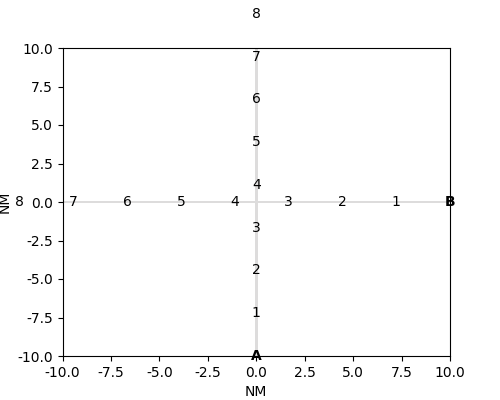
\includegraphics[width=0.75\textwidth,height=0.75\textheight,keepaspectratio]{../src/img/crossing.png}
    \caption{Crossing scenario}
    \label{fig:simple-scen}
\end{figure}

The first scenario depicts a simple crossing situation where two vessels are on perpendicular courses. The vessels start  approximately 14 NM from each other with a speed of 10 kts as seen in figure \ref{fig:simple-scen}. The vessels maximum speed is set to 12 kts and maximum rate of turn \ang{3} per second. The two vessels are to  collide in origo if no corrections are made to either course or speed. COLREGs \textit{rule 15} stipulate that vessel (\textit{A}) that has the other vessel on its starboard side  in a crossing situation should alter its course to starboard, thereby, avoiding passing in front of the other vessel (\textit{B}).
\begin{figure}[H]
    \centering
    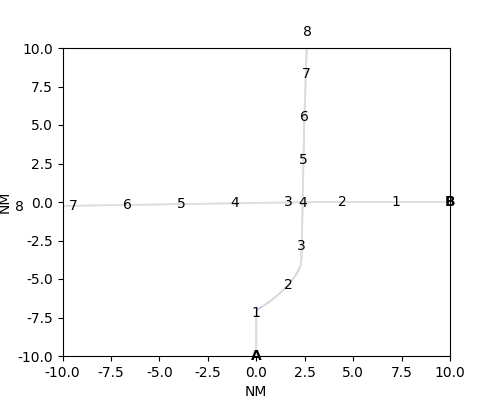
\includegraphics[width=0.75\textwidth,height=0.75\textheight,keepaspectratio]{../src/img/crossing_res.png}
    \caption{Crossing scenario}
    \label{fig:simple-scen-res}
\end{figure}

Figure \ref{fig:simple-scen-res} shows the scenario when both boats are guided by the FIS system. The numbers on the vessels tracks are printed every thousand seconds, which equal 16 minutes and 40 seconds, and help to compare the vessels positions at  given time frames. These numbers will from here on be referred to with bold numbers.

It can be seen that both vessels continue along their original paths until vessel \textit{A} reaches \textbf{1}, at which point the distance to vessel \textit{B} has shrunk to 10NM and the algorithm becomes aware of the target vessel. Vessel \textit{A} will at this point initiate a starboard turn  of \ang{24}  to pass behind vessel \textit{B} as specified in COLREGs. Vessel \textit{A} will then follow headings suggested by the ANS until \textbf{2.7} where  vessel \textit{B} is no longer considered a threat, i.e. no rule in the FIS applies, after which it steers back to its original heading. Vessel \textit{B} will during the whole scenario be the stand on vessel and, therefore, keep its course and speed.

The ANS suggestions are exactly as described in the COLREGS documents for this case. The manoeuvre is initiated at a distance of 10 NM, which can be regarded as ample time (\textit{Rule 8}). The correction is, furthermore, large and therefore clearly visible to the other vessels involved.

\section{Overtaking and head-on scenario}%-------------------------------------------
%------------------------------------------------------------------------------------


\begin{figure}[H]
    \centering
    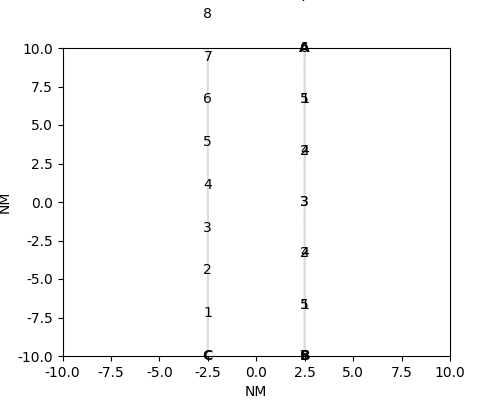
\includegraphics[width=0.75\textwidth,height=0.75\textheight,keepaspectratio]{../src/img/overtaking_head_on.png}
    \caption[Overtaking and head-on scenario]{Overtaking and head-on scenario  \cite{ecolreg_overtaking-and-head-on}}
    \label{fig:overtaking-and-head-on}
\end{figure}
This scenario defines a three vessel scenario, where two vessels are meeting on  reciprocal courses. One of the vessels is, furthermore, overtaking a third vessel on the stand on vessels starboard side. A visualization of the scenario is shown in figure \ref{fig:overtaking-and-head-on}. Vessels \textit{A} and \textit{B} starts on reciprocal tracks 20 NM from each other, while \textit{B} and \textit{C} start abreast 5 NM from each other. \textit{A}, \textit{B}, and \textit{C} has a maximum speed of 15 kts. \textit{A} and \textit{B} start at 12 kts while \textit{C} is slightly slower at 10 kts. Maximum rate of turn of all vessels is set to \ang{3} per second.

Vessels \textit{A} and \textit{B} are obliged to alter their courses to starboard to prevent a head-on collision (\textit{Rule 14}). Moreover, vessel \textit{B} shall keep out of the way of \textit{C}  and in no circumstance alter its course so that it becomes a crossing vessel to \textit{C} (\textit{Rule 13}). All corrections shall furthermore be ample, so that it is recognizable by the other vessel, and taken as early as possible (\textit{Rule 16}) \cite{ecolreg_overtaking-and-head-on}.

\textcite{ecolreg_overtaking-and-head-on} suggest that vessel \textit{A} should alter course to starboard and pass ahead of vessel C,  to avoid a collision.



\begin{figure}[H]
    \centering
    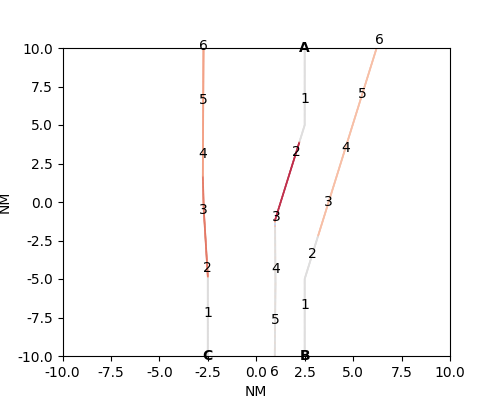
\includegraphics[width=0.75\textwidth,height=0.75\textheight,keepaspectratio]{../src/img/overtaking_head_on_res.png}
    \caption{Overtaking and head-on scenario  }
    \label{fig:overtaking-and-head-on-res}
\end{figure}
The same initial scenario with the ANS enabled can be seen in figure \ref{fig:overtaking-and-head-on-res}. Vessels \textit{A} and \textit{B} are the first vessels to make alterations to their initial states. Both initiate starboard turns   at \textbf{1.5} to avoid colliding head-on. Vessel \textit{B} continues on that course for the rest of the scenario, while vessel \textit{A} steers back to its original course at \textbf{3} when it has passed vessel \textit{C}. Vessels \textit{C} and \textit{A} will at \textbf{1.8} accelerate since they both have each other in sector \textit{II} with a relative course in sector \textit{e} and are therefore in a head-on situation.

The ANS simulation does not result in the same manoeuvres as recommended by \textcite{ecolreg_overtaking-and-head-on}, since vessel \textit{A} is passing between the two other vessels instead of ahead of vessel \textit{C}. This might to some extent be due to the spacing between the vessels on the X-axis at the start of the scenario. A 5 NM spacing was chosen since the $R_b$ radius is set to 4 NM. The vessels where able to pass each other at safe distance, but the solution involves  more vessels making alterations to their courses than the recommended one. The speed alterations could also be considered unnecessary. The speed alterations comes directly from the rule-set and can therefore probably be improved by fine tuning the rules. However, the amount of alterations, stems from the fact that vessel \textit{A} starts its first one at \textbf{1.5}, when vessel \textit{C} is still outside of its range and therefore unknown to vessel \textit{A}. Vessel \textit{A} will become aware of vessel \textit{C} at \textbf{1.8}, when vessel \textit{C} has already passed from sector I to II, and vessel \textit{A} will, therefore, accelerate instead of turning further to the right.

The solution presented in figure \ref{fig:overtaking-and-head-on-res}, although different from the one recommended by \textcite{ecolreg_overtaking-and-head-on} succeed in keeping the vessel from colliding. All course changes are additionally, correct according to the COLREG rules. The speed changes are however, accelerations instead of decelerations as described in  \textit{rule 8}.


\section{Overtaking and crossing scenario 1}%----------------------------------------
%------------------------------------------------------------------------------------


\label{sec:overtaking-and-crossing}
\begin{figure}[H]
    \centering
    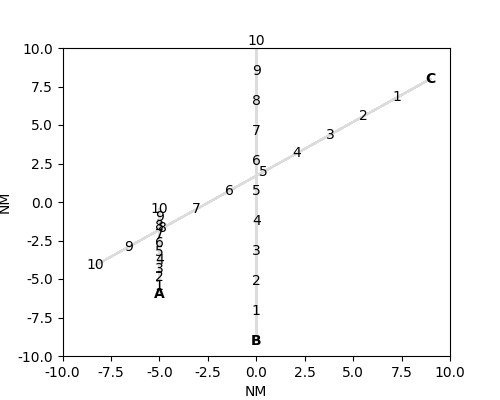
\includegraphics[width=0.75\textwidth,height=0.75\textheight,keepaspectratio]{../src/img/overtaking_crossing.png}
    \caption[Overtaking and crossing scenario 1]{Overtaking and crossing scenario 1 \cite{ecolreg_overtaking-and-crossing}}
    \label{fig:overtaking-and-crossing}
\end{figure}
The three following scenarios all depict scenarios where vessels \textit{A} and \textit{B} are in an overtaking situation while \textit{C} crosses both their paths. \textit{C} crosses \textit{A} and \textit{B}s paths with a \ang{45}  angle in the first scenario (figure \ref{fig:overtaking-and-crossing}). \textit{A} starts at (-5, -6), \textit{B} at (0, -9) and \textit{C} in (9, 8). \textit{A} and \textit{B} has an initial heading of \ang{0}  while \textit{C} start with a heading of \ang{235}. The speeds of the vessels is set to ensure that \textit{C} will collide with both vessels if no corrections are applied. Moreover, the speed of \textit{B} must be greater than the speed of \textit{A} since \textit{B} is overtaking \textit{A}. The vessels initial speed are, therefore: \textit{A} = 2 kts, \textit{B} = 7 kts and \textit{C} = 7.6 kts. The maximum speeds of the vessels are 10, 15 and 20 kts respectively. Maximum rate of turn of all vessels is set to \ang{3} per second.

Rule 13 and 16 apply to this scenario in the same way as the previous one, with the exception that the vessels involved in the overtaking situation is vessel \textit{A} and \textit{B} instead of \textit{B} and \textit{C}. This implies that \textit{B} shall keep out of way of \textit{A} (\textit{Rule 13}), while \textit{A} shall keep its course and speed (\textit{Rule 17}).

Additionally, both \textit{A} and \textit{B} are crossing \textit{C}s path with a risk of collision. This means that \textit{A} and \textit{B} should alter their courses to starboard and avoid passing in front of \textit{C} (\textit{Rule 15}). Vessel \textit{C} shall, meanwhile, keep its course and speed. This results in contradictory obligations for vessel  \textit{A}, where it should keep its course and speed for \textit{B} and simultaneously keep out of the way for vessel \textit{C}.

\textcite{ecolreg_overtaking-and-crossing} suggest the following manoeuvres for vessel \textit{A} and \textit{B} in accordance with the ordinary practice of seamen:
Both vessels might alter course to starboard and, thereby, pass behind vessel \textit{C}. Alternatively vessel \textit{A} may reduce speed or make a \ang{360} turn to port, while vessel \textit{B} reduces speed, makes a \ang{360} to starboard or alters its course to starboard.

\begin{figure}[H]
    \centering
    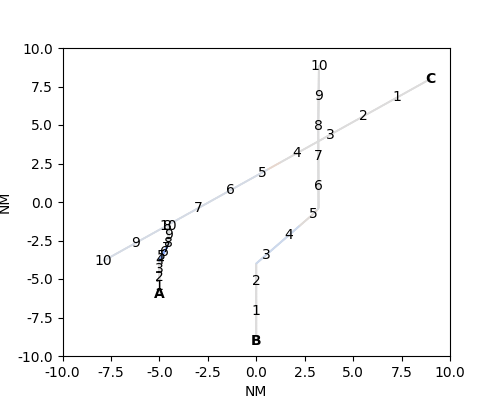
\includegraphics[width=0.75\textwidth,height=0.75\textheight,keepaspectratio]{../src/img/overtaking_crossing_res.png}
    \caption{Overtaking and crossing scenario 1}
    \label{fig:overtaking-and-crossing-res}
\end{figure}

The recommendations by the ANS matches the ordinary practice of seamen quite well for this scenario. Vessel \textit{A} chooses to slow down and alter its course slightly to starboard, while vessel \textit{B} alters its course to starboard. Thus vessel \textit{A} made two corrections instead of one as recommended.  The vessels manage to keep a safe distance and none of the stand on vessels are forced to alter their courses. Vessel \textit{C} keeps its original heading and course during the whole simulation. A visualization can be seen in figure \ref {fig:overtaking-and-crossing-res}.

\section{Overtaking and crossing scenario 2}%----------------------------------------
%------------------------------------------------------------------------------------


\begin{figure}[H]
    \centering
    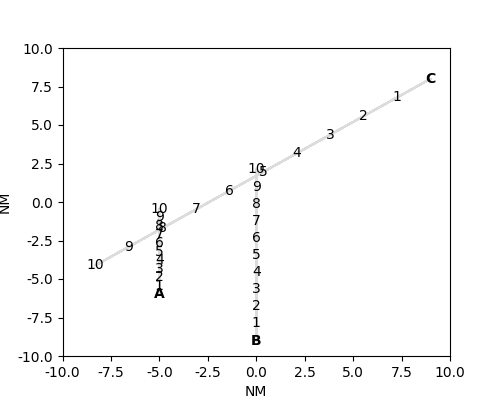
\includegraphics[width=0.75\textwidth,height=0.75\textheight,keepaspectratio]{../src/img/overtaking_crossing_3.png}
    \caption[Overtaking and crossing scenario 2]{Overtaking and crossing scenario 2 \cite{ecolreg_overtaking-and-crossing-3}}
    \label{fig:overtaking-and-crossing-3}
\end{figure}
The next scenario, visualized in figure \ref{fig:overtaking-and-crossing-3}, differs from the previous only in that B and C are not at risk of collision since Bs speed is decreased to 4 kts. This means that B has no obligations to alter its course to starboard to avoid C as in the previous scenario. All other rules from the previous scenario do apply and vessel A is, therefore, still in the contradictory situation where it shall both keep course and speed for vessel B and alter course to starboard to avoid vessel C.

The following actions by vessel A solve the situation in accordance with the ordinary practice of seamen. It might either slow down, make a 360 degree turn to port or alter course to starboard and pass in front of vessel B if time permits.



\begin{figure}[H]
    \centering
    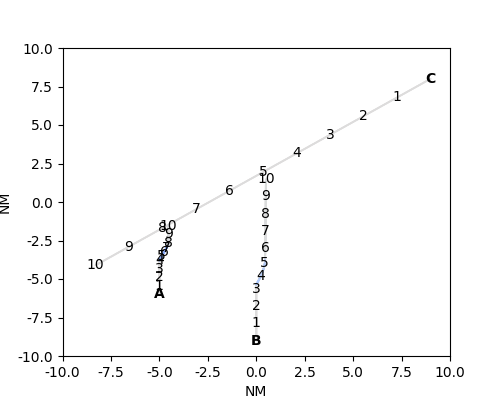
\includegraphics[width=0.75\textwidth,height=0.75\textheight,keepaspectratio]{../src/img/overtaking_crossing_3_res.png}
    \caption{Overtaking and crossing scenario 2}
    \label{fig:overtaking-and-crossing-3-res}
\end{figure}

This scenario is almost identical to the previous with the exception that there is no risk of collision between vessel \textit{B} and \textit{C}. These vessels should therefore, ideally not make any alterations to their courses. However, vessel \textit{A} has to avoid vessel \textit{C}, which is coming from starboard. Figure \ref{fig:overtaking-and-crossing-3-res} shows how vessel \textit{A} both alters course and slows down as in the previous scenario, which causes vessel \textit{B} to also alter its course to starboard to avoid vessel \textit{A}. This manoeuvre by vessel \textit{B} is completely unnecessary since vessel \textit{As} speed is significantly lower than \textit{B's} and a collision is, therefore, not imminent even thought vessel \textit{A} turns towards vessel \textit{B}.

\section{Overtaking and crossing scenario 3}%----------------------------------------
%------------------------------------------------------------------------------------


\begin{figure}[H]
    \centering
    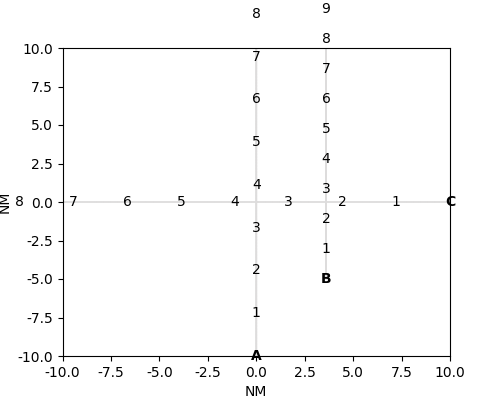
\includegraphics[width=0.75\textwidth,height=0.75\textheight,keepaspectratio]{../src/img/overtaking_crossing_2.png}
    \caption[Overtaking and crossing scenario 3]{Overtaking and crossing scenario 3 \cite{ecolreg_overtaking-and-crossing-2}}
    \label{fig:overtaking-and-crossing-2}
\end{figure}

The last scenario depicts a similar scenario as the previous two, with two vessels in an overtaking situation while a third cross their paths. The scenario is visualized in figure \ref{fig:overtaking-and-crossing-2}. Vessel \textit{A} starts at (0, -10), vessel \textit{B} at (3.6, 5) and \textit{C} at (10, 0). The two vessels involved in the overtaking situation, that is \textit{A} and \textit{B}, start with a heading of \ang{0}  while  \textit{C} starts with a {270} heading in order to cross the two other vessels paths perpendicularly. \textit{A} and \textit{C} start at a speed of 10 kts while \textit{B} starts at 15 kts. All vessels have as maximum speed of 20 kts and a maximum rate of turn of \ang{3} per second. The same rules apply as in the two previous rules, but the manoeuvring space for vessels \textit{A} and \textit{B} is slightly more limited due to the angle which C approaches on.

Vessel \textit{A} is also in this scenario in a situation where two rules contradict each other.
It shall keep course and speed for vessel \textit{B} while simultaneously avoiding vessel \textit{C}.
Vessel \textit{C} shall keep course and speed for both vessel \textit{B} and \textit{A}.
Finally vessel \textit{B} shall keep out of the way of vessel \textit{A} and alter course to starboard to avoid vessel C.

One of the following actions is recommended to avoid collisions \cite{ecolreg_overtaking-and-crossing-2}. Both vessels might alter their course to starboard and pass behind vessel \textit{C} to avoid collision. The action must however be initiated by vessel \textit{B}. Alternatively vessel \textit{A} might either reduce speed or make a 360 degree turn. The turn must be initiated early if made to starboard. Vessel \textit{B} must at the same time also reduce speed, make a \ang{360} turn to starboard or alter course to starboard to avoid colliding with vessel \textit{C}



\begin{figure}[H]
    \centering
    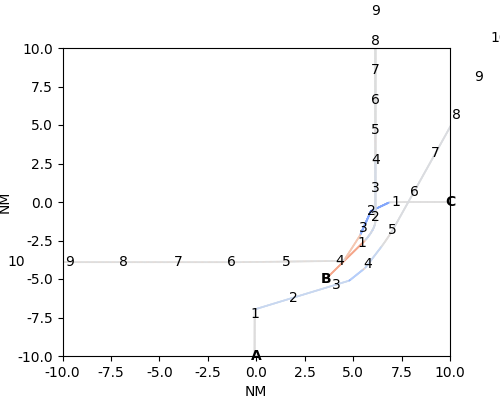
\includegraphics[width=0.75\textwidth,height=0.75\textheight,keepaspectratio]{../src/img/overtaking_crossing_2_res.png}
    \caption{Overtaking and crossing scenario 3}
    \label{fig:overtaking-and-crossing-2-res}
\end{figure}

The ANS simulation starts out as described above with vessels \textit{A} and \textit{B} altering courses to starboard to pass behind vessel \textit{C}. Additionally Vessel A slows down while vessel \textit{B} accelerates. The two vessels avoid each other exactly as described by \textcite{ecolreg_overtaking-and-crossing-2}, apart from the extra speed changes. However, the alterations made by vessel \textit{B} to avoid void vessel \textit{C} and \textit{A} make the distance between vessel \textit{B} and \textit{A} shrink to under $R_b$, which forces vessel \textit{C} to alter its course to port and decrease its speed. This causes vessels \textit{B} to steer towards vessel \textit{C}, thereby increasing the collision risk between the two vessels and breaking the COLREG rules. However, it could be argued that the initial placement of the vessels does not correspond to a normal situation since vessel \textit{B} and \textit{C} start at a distance less than $R_a$ and therefore have limited manoeuvring space.


\chapter{Discussion}%----------------------------------------------------------------
%------------------------------------------------------------------------------------
\label{chap:disc}
The goal of this thesis has been to further examine the work of \textcite{perera2012intelligent}, regarding the use of fuzzy logic to facilitate collision avoidance amongst USVs. The previous research presents successful results in
basic multi vessel situations at sea. However, only one of the vessels featured in the scenarios of that paper uses FIS to navigate. The other vessels
are dummy vessels that keep their speed and course for the whole scenario.
The contribution of this thesis would, therefore, be to test the usage of a FIS
based ANS in scenarios where multiple vessels navigate uses it. Such scenarios put the vessels in situations where they are simultaneously supposed to give way and stand on and thereby has to prioritize the actions suggested by the ANS. An average weighted on expected collision time is used to prioritize the FIS recommended actions, rather
than Bayesian networks, as suggested by \textcite{perera2012intelligent}.

The results of the simulations presented in section \ref{sec:evaluation} show that the FIS based ANS manages to prevent collision in all of the scenarios. Although the corrections made by the vessels were not always in accordance with the ordinary practice of seamen. For instance, the scenarios depicted in figures \ref{fig:overtaking-and-head-on-res} and \ref{fig:overtaking-and-crossing-2-res} show vessels accelerating although the COLREG rules only mention decreasing the speed as a proper response in case of an impending collision. This can to some extent be blamed on the configuration of the FIS, i.e the  antecedents and consequents, as well as the rules, specified. The previously mentioned example stems from a rule with acceleration as a consequent.  The FIS configuration is in other words crucial to the quality of the ANS system. The possibility to simply define rules was one of the reasons why fuzzy logic was initially chosen for this thesis since such a system would enable people with navigation expertise to verify the rules even though they do not understand the underlying technology. This would potentially facilitate the process to certify the algorithm as safe. However, a large rule-set  and multiple inputs might quickly become difficult to comprehend since the change in one rule might have implications on how another vessel acts in  certain scenarios. This situations is further complicated by the fact that the parameters would have to be adjusted to suit the particular vessel type the ANS system is a part of. Additionally different rule sets would probably have to be designed for different situations. The scenarios is this thesis are all set on the open sea, while many of the COLREG rules specify more specific situations. This could result in quite large rule-sets, that might be tedious to verify and maintain.

Another issue that needs to be considered is the way the current system defines visible target vessels. This becomes particularly evident in figure \ref{fig:overtaking-and-crossing}, where vessel \textit{B} reaches vessel \textit{A}'s $R_A$ slightly before vessel \textit{C}. This results in vessel \textit{A} accelerating instead of turning further to the right. This situation could possibly be improved by redesigning the range FMF, so that the membership value increases gradually as the vessels approach each other. The current FMF goes from zero to one as the target vessel passes $R_A$. Increasing the fuzzy area of the FMF past $R_A$ with a gradual decrease towards zero could potentially increase the vessels SA, thereby enabling it to make better decisions.

Furthermore, some of the corrections suggested by the ANS could be considered unnecessary. For instance vessel \textit{B's} course change in figure \ref{fig:overtaking-and-crossing-3-res}. COLREGs \textit{rule 7} state that a collision is imminent when two vessels have constant compass bearing over a prolonged time, which is not the case in figure \ref{fig:overtaking-and-crossing-3-res}. The current system lacks this kind of comparison between the  current situation and a previous instance and is therefore, unable to comply with \textit{7}. This might lead to unnecessary corrections and could potentially trigger chain reactions between USV's in range of each other.


\chapter{Conclusions}%---------------------------------------------------------------
\label{chap:conc}

Successful development of USVs able to safely navigate among both other USV and ordinary manned vessels could, apart from being safer,  decrease the operational costs of the maritime shipping industry significantly. However, collision avoidance systems for USVs can be implemented in a variety of ways. The purpose of this thesis has been to evaluate the FIS based collision avoidance algorithm presented by \textcite{perera2012intelligent,perera2010smooth_param}, by reimplementing it in python and increasing the complexity of the tested simulation scenarios. Furthermore, an analysis of the COLREG rules and the fuzzy logic elements used in the algorithm was made in order to reimplement the algorithm and  develop a simulation framework.

Both the research by \textcite{perera2012intelligent,perera2010smooth_param}  and this thesis prove that the developed FIS based ANS do manage to avoid collision between USVs in basic COLREG situations. However, the more complicated scenarios  reveal a few limitations in the algorithm. The decisions made by the algorithm will, for instance, not always follow ordinary practice of seamen and could therefore confuse the crew of manned vessels. Mostly due to the fact that the current implementation  only analyses the present situation and is therefore unable to make decisions based on comparison to previous states.

An initially appealing aspect of the fuzzy logic based solution was the ability to write the navigation logic as IF-THEN based rules, thereby facilitating verification of the algorithm by people not familiar with the underlying logic. However, designing a maintainable and efficient  rule-set could prove complicated. For instance, most of the non COLREGs compliant corrections suggested during the simulations stem from poorly defined rules.





%------------------------------------------------------------------------------------
% Works but might not be the most effecient
% Intheory easy to verify rules

\section{Further work}%--------------------------------------------------------------
%------------------------------------------------------------------------------------
The two major limitations found during the evaluation are, as stated in the previous section, the rule-set and the algorithms inability to make decisions based on a holistic model of the situation.
Further analysis of the rule-set and its corresponding antecedents and consequents is, therefore, needed to ensure safe decisions in all situations. Moreover, improvements should be considered to ensure that the decisions made by the ANS follows ordinary practice of seamen. This improvement includes both rule changes as well as an upgrade to the way multi target situations are prioritized.
Finally system needs to be incorporated into a full ANS with real SA and navigation modules for further testing and simulations.
% Improve rules
% Add way to compare time frames
%Different vessels (fishing, tow, mm)

%\include{Chapters/Chapter5} 

%----------------------------------------------------------------------------------------
%   THESIS CONTENT - APPENDICES
%----------------------------------------------------------------------------------------

\appendix % Cue to tell LaTeX that the following "chapters" are Appendices

% Include the appendices of the thesis as separate files from the Appendices folder
% Uncomment the lines as you write the Appendices

% Appendix A

\chapter{Frequently Asked Questions} % Main appendix title

\label{AppendixA} % For referencing this appendix elsewhere, use \ref{AppendixA}



%!TEX root = ../main.tex
% !TeX spellcheck = en_GB 
% Appendix A

\chapter{Python Code} % Main appendix title
\label{chap:python_code} % For referencing this appendix elsewhere, use \ref{AppendixA}


\begin{listing}
    \inputminted[linenos, breaklines=true,fontsize=\scriptsize, numberblanklines=false]{python}{Appendices/rel_bear.py}
    \caption{Methods used to calculate the relative bearing from a ship to another from their heading and Cartesian coordinates}
    \label{listing:rel_bear_calc}
\end{listing}
%\include{Appendices/AppendixC}
\begin{otherlanguage}{swedish}
    %!TEX root = ../main.tex
% !TeX spellcheck = en_GB
% Appendix Template
\addtocontents{toc}{\protect\setcounter{tocdepth}{0}}
\renewcommand{\thesection}{\arabic{section}}
\addchap{Svensk sammanfattning} % Main appendix title
\label{app:swed_sum} % Change X to a consecutive letter; for referencing this appendix elsewhere, use \ref{AppendixX}

\addsec{Introduktion}
Maritim frakt kan ses som en av grundpelarna i den moderna ekonomin, eftersom upp till 90\% av dagens frakt går sjövägen \cite{percent_trade}. Den senaste tidens stora framsteg inom sensorteknologi och artificiell intelligens har väckt intresset för utveckling av obemannade fartyg. Dylika fartyg skulle  potentiellt kunna minska de operationella kostnaderna för maritima operationer och samtidigt minska antalet olyckor \cite{manley2008unmanned,marine_casualities_incidents_2017}. Det är därför av yttersta intresse för den maritima industrin att överkomma de utmaningar som obemannade fartyg för med sig. En av dessa utmaningarna är att få fartygen att följa nuvarande sjöfartsregler. Denna avhandling  evaluerar användningen av suddig logik som bas till en algoritm för kollisionsundvikande till sjöss enligt  de internationella sjövägsreglerna (Konvention om de internationella reglerna till förhindrande av sammanstötning till sjöss, 1972) \cite{colreg}.
\addsec{Obemannade fartyg}
Utvecklingen av autonoma fartyg har redan pågått i flera decennier och flera olika metoder samt algoritmer har utvecklats och evaluerats. Majoriteten av projekt har dock resulterat i semi-autonoma fartyg. Semi-autonoma fartyg innebär att en person kan övervaka ett flertal autonoma båtar från land och fjärrstyra dem vid behov. Det betyder att fartyg kan byggas utan en bemannad brygga, duschar, kantin och andra dylika faciliteter som krävs om människor skall vistas ombord under längre tider. Operationella kostnaderna kunde emellertid minskas ännu mer ifall fartygen kunde göras totalt autonoma och inte kräva en övervakare. För att klara detta krävs algoritmer med samma beslutsfattningsförmåga som de mänskliga operatörerna. Denna avhandling koncentrerar sig på beslut angående kollisionsundvikande och antar därför att det autonoma fartyget har full situationsmedvetenhet.
\addsec{De internationella sjövägsreglerna}
Alla fartyg som navigerar på öppna havet och alla vatten tillknutna därtill är tvungna att följa de internationella sjövägsreglerna. Detta gäller också autonoma fartyg. Reglerna är dock skrivna 1972 och för att tolkas av människor, vilket medför utmaningar när dessa skall tolkas av maskiner.

De internationella sjövägsreglerna är uppdelade i fem delar, varav delarna ett till tre är av intresse för denna avhandling. Längden av detta sammandrag tillåter dessvärre inte mer än en genomgång av de regler som är essentiella för kollisionsundvikande, nämligen reglerna 7-17. Dessa definierar kriterierna för vad som klassas som kollisionsrisk samt rekommenderade hastighets och kursändringar vid kollisionsrisk. Vidare specificeras tre scenarion och fartygs roller och obligationer i scenariot i fråga. Scenarierna är upphinnande, stäv emot stäv och skärande kurser. Vid upphinnande skall fartyget med högre fart ändra sin kurs och passera det andra fartyget på endera babord eller styrbord sida. I ett stäv mot stäv scenario skall bägge fartyg korrigera sin kurs till styrbord. Slutligen skall i ett scenario med skärande kurser fartyget med det andra fartyget på styrbord sida korrigera sin kurs mot styrbord. I samtliga scenarier är det andra fartyget ålagt att hålla sin kurs och hastighet \cite{colreg}. I verkligheten är oftast flera fartyg inblandade i dessa situationer och fler regler kan därför vara aktiva samtidigt. I sådana situationer krävs ett helhetsbeslut baserat på gott sjömanskap, vilket är en utmaning för autonoma fartyg.


\addsec{Suddig logik}
Suddig logik utvecklades av \textcite{zadeh1996fuzzy} 1964 och är en gren av logik där propositioner kan vara delvis sanna. Sanningsvärden kan således vara alla reella tal från 0 till 1. Detta för att  enklare kunna efterlikna mänskans abstrakta resonemang.  Det är därmed möjligt att definiera mängder så som  \textit{långa personer}  där objektets medlemskapsvärde beror av hur mycket personens längd avviker från det normala \cite{chen2000introduction}.  Graden av medlemskap för \textit{a} i den suddiga mängden $\fuzzyset{A}$ bestäms av den suddig medlemskapsfunktionen $\mu_{\fuzzyset{A}}(a)$.   Figur \ref{fig:FMF_ex} visar en enkel suddig medlemskapsfunktion för mängden \textit{gamla personer}. En ålder av 90 år ger i detta exempel medlemskapsvärdet 80.

Suddig logik möjliggör  modellering av komplexa system, som vanligtvis är beskrivna med naturligt språk och skrivet för att tolkas av människor. Dylika system kan ofta beskrivas med regler av följande form :

\begin{equation}
    \text{OM premiss , SÅ slutsats}
\end{equation}



\addsubsec{Modell för de internationella sjövägsreglerna}
Denna avhandling baserar sig på en tidigare utvecklad modell av \textcite{perera2010smooth_param,perera2012intelligent}. Modellen består av ca 200 regler, som i sin tur har fyra premisser och två slutsatser var.  Premisserna är relativ bäring från huvudfartyget till målfartyget, målfartygets relativa kurs, distansen mellan fartygen och förhållandet mellan deras hastigheter. De suddiga medlemskapsfunktionerna för premisserna och slutsatserna visualiseras i figurerna \ref{fig:antecedent_fmfs} och \ref{fig:consequent_fmfs}.  I denna avhandling används Mamdanis  slutledningsmetod för att räkna ut ett numeriskt värde för slutsatserna utgående från regelverket, de suddiga medlemskapsfunktionerna och  premissernas numeriska värden.


\addsec{Implementering}
<<<<<<< Updated upstream
För att evaluera användningen av suddig logik vid kollisionsundvikande utvecklades ett suddigt slutledningssystem samt ett ramverk för att simulera situationer som beskrivs i de  internationella sjövägsreglerna. Bägge är implementerade i Python. Slutledningssystemet använder sig av python-biblioteket SciKit-Fuzzy \cite{josh_warner_2017_1002946} för uträkning av kurs och hastighetsändringar utgående från  de för tillfället rådande premisserna. Simuleringen utspelar sig i ett tvådimensionellt kartesiskt koordinatsystem där fartyg representeras av punkter med  kurs och hastighet. Varje fartyg har definierade gränser för max hastighet, svängradie, acceleration och retardation.  Ett tvådimensionellt koordinatsystem valdes eftersom simuleringen inte tar i beaktande väderfenomen. Simulationen uppdateras med en sekunds intervall, varpå  korrektioner för kollisionsundvikande appliceras och fartygens position uppdateras enligt deras momentanhastighet och kurs.   Eftersom situationer kan innefatta fler fartyg och därmed fler regler krävs ett system för att prioritera korrigeringsförslagen. I denna avhandling görs detta med hjälp av viktat aritmetiskt medelvärde. Medelvärdet av alla korrigeringar viktas enligt tid till kollision, baserat på  distansen mellan fartygen och deras relativa hastighet.



\addsec{Evaluering och slutsats}

För att testa systemet för kollisionsundvikande konstruerades fem olika scenarier. Fyra av dessa involverar tre fartyg medan det första endast involverar två fartyg på skärande kurser.  Av de fyra andra scenarierna är tre av typen upphinnande och skärande, i vilket ett fartyg hinner upp ett annat samtidigt som ett tredje fartyg korsar dess väg . Det sista scenariot visar en situation där ett fartyg hinner upp ett annat samtidigt som ett tredje fartyg möter det upphinnande fartyget stäv mot stäv.  Scenarierna baserar sig på scenarier från \textcite{ecolreg_overtaking-and-crossing,ecolreg_overtaking-and-crossing-3,ecolreg_overtaking-and-crossing-2,ecolreg_overtaking-and-head-on}.  Simulationer av scenarierna visar att systemet tar beslut i  enlighet med   internationella sjövägsreglerna vid enkla situationer som endast innefattar en regel.  Kollision undveks också i de scenarier som involverade fler fartyg och därmed regler. Kurs och hastighetskorrigeringarna var däremot inte alltid i enlighet med sjövägsreglerna. Figurerna \ref{fig:overtaking-and-head-on-res} och \ref{fig:overtaking-and-crossing-3-res} visar att fartygen ökat hastigheten för att undvika kollision, medan sjövägsreglerna endast nämner sänkning av hastigheten som en lämplig korrigering. Vidare kan konstateras att antalet korrigeringar ofta blir onödigt högt  eftersom systemet inte klarar av att ta beslut baserat på en fullständig helhetsbild.  Onödiga korrigeringar kan förbrylla manskap vid bemannade fartyg och  autonoma system ombord på andra fartyg.

Felaktiga korrigeringar så som  hastighetsökning istället för sänkning kan till viss mån  bero på dåligt specificerade regler. I detta fall är hastighetsökning med som slutsats i ett flertal regler i regelverket. Syftet med denna avhandling var dock endast att evaluera en befintligt lösning och ändringar i regelverket är därför utanför dess omfattning. Möjligheten att definiera klara OM-SÅ regler, var emellertid en av orsakerna till att just denna algorithm valdes för evaluering.  Vidare forskning är dock  nödvändig för att revidera regelverket och möjligtvis premisserna.


Slutligen konstateras att ytterligare utveckling krävs för att garantera att korrigeringsförslagen är i enighet med  gott sjömanskap för att undvika tvetydigheter. Detta innefattar både revidering av regelverk och bättre hantering av situationer som innefattar fler än två fartyg. Ytterligare testning, gärna integrerat med riktiga moduler för navigering och situationsmedvetenhet, ses också som nödvändigt.
\end{otherlanguage}
%----------------------------------------------------------------------------------------
%   BIBLIOGRAPHY
%----------------------------------------------------------------------------------------

\printbibliography[heading=bibintoc]

%----------------------------------------------------------------------------------------

\end{document}
